\documentclass[acmlarge]{acmart}



\AtBeginDocument{%
  \providecommand\BibTeX{{%
    Bib\TeX}}}
  \settopmatter{printacmref=false}

\renewcommand{\descriptionlabel}[1]{\hspace{\labelsep}\textit{#1}}
\usepackage{xcolor}
\usepackage{multicol}
\usepackage{geometry}
\newcommand{\todo}{{\color{red}\textbf{TODO} }}
\newcommand{\disease}{{\small \texttt{DISEASE}} }
\newcommand{\hospital}{{\small \texttt{HOSPITAL}} }
\newcommand{\storage}{{\small \texttt{STORAGE}} }

% christos 2, 4
% vasilis 1, 3

\usepackage{amsmath}
\usepackage{subfig}

\usepackage{hyperref}
\usepackage{algorithm}
\usepackage{algpseudocodex}
\newcommand{\algorithmautorefname}{Algorithm}

\begin{document}

\title{Big Data Analytics with Scala and Apache Spark}
\subtitle{M.Sc. course on ``Technologies for Big Data Analysis'' - Assignment 3}

\author{Christos Balaktsis (506)}
\email{balaktsis@csd.auth.gr}
\author{Vasileios Papastergios (505)}
\email{papster@csd.auth.gr}
\affiliation{
  \institution{Aristotle University}
  \city{Thessaloniki}
  \country{Greece}
}

\renewcommand{\shortauthors}{C. Balaktsis and V. Papastergios}
\maketitle

\section{Introduction}

The current document is a technical report for the third programming assignment in the M.Sc. course on
\emph{Technologies for Big Data Analysis}, offered by the \emph{DWS M.Sc Program}\footnote{https://dws.csd.auth.gr/} of the Aristotle University of Thessaloniki, Greece. The course is taught by Professor Apostolos Papadopoulos~\footnote{https://datalab-old.csd.auth.gr/$\sim$apostol/}. The authors attended the course during their first year of Ph.D. studies at the Institution.

The assignment contains 4 sub-problems and is part of a series, comprising 3 programming assignments on the following topics:
\begin{description}
  \item[Assignment 1] Multi-threading Programming and Inter-Process Communication
  \item[Assignment 2] The Map-Reduce Programming Paradigm
  \item[Assignment 3] Big Data Analytics with Scala and Apache Spark
\end{description}
In this document we focus on Assignment 3 and its 4 sub-problems.
We refer to them as \emph{problems} in the rest of the document for simplicity.
The source code of our solution has been made available at the following public repository in the GitHub platform: \href{https://github.com/Bilpapster/big-data-playground}{\texttt{\small https://github.com/Bilpapster/big-data-playground}}.

\textbf{Roadmap}.
The rest of our work is structured as follows.
We devote one section to each one of the 4 problems.
That means problems 1, 2, 3 and 4 are presented in~\autoref{sec:problem1},~\autoref{sec:problem2},~\autoref{sec:problem3} and~\autoref{sec:problem4} respectively.
For each problem, we first provide the problem statement, as given by the assignment.
Next, we thoroughly present the reasoning and/or methodology we have adopted to approach the problem and devise a solution.
Wherever applicable, we also provide insights about the source code implementation we have developed.
Finally, we conclude our work in~\autoref{sec:conclusion}.
The appendix includes the evaluation results for any issues that necessitated them.

\section{Problem 1: Word Length Analytics}
\label{sec:problem1}
We discuss here the first problem of the assignment.
The main target of the assignment is to get familiar with a simple task leveraging Apache Spark and Scala programming language. This is a WordCount problem's variation.

\subsection{Problem Statement}
Implement an \textbf{Apache Spark} (Scala) program, a variation of the \textbf{word-count} problem, to compute the average length of words that start with a specific letter (a-z). The program should sort the results based on the average length, printing first the letters with higher average length. For example:
\begin{description}
  \item k – $8.2$
  \item a – $5.6$
  \item b – $4.8$
\end{description}
Note that you may opt for preprocessing the input text, e.g., transforming all letters to lowercase or ignoring words that start with a number.

\subsection{Proposed approach}
\subsubsection{Setting}
Our implementation is run and tested in a Linux environment with 12 cores, using the Scala programming language version 2.13.15 and Apache Spark version 3.5.3. We have used SBT as the build tool of our solution.
We have used the Software Development Kit (JDK) version 11.0.11.
The source code is developed in IntelliJ IDEA Community Edition 2021.1.1 and managed using SBT as the build tool. All dependencies of the project can be found in the \texttt{build.sbt} file located at the root folder of the project.
The project is compiled and executed directly from the IntelliJ IDEA.

To run the project, open the \texttt{src/main/scala/Task1WordLength.scala} file in IntelliJ IDEA, and execute the main method. After successful execution of the program, the results can be viewed under the \texttt{output/task1} directory.

\subsubsection{Implementation}
The proposed approach leverages the Apache Spark computing framework to calculate the average word length for each one of the 26 letters in the Latin alphabet. In particular, the input text is read and tokenized into words. As part of a preprocessing step, all letters are transformed to lowercase and all words that start with a number are dropped.

In order to compute the average length for each initial letter, we leverage the \texttt{RDD} API of Apache Spark. More specifically, we use a \texttt{PairRDD} that stores composite key-value pairs in the form \texttt{(letter, (word\_length, 1))}. The key of each pair is the initial letter of the respective word (\texttt{letter}). The value of each pair is a pair itself, having as (false) key the length of the word (\texttt{word\_length}) and as (false) value a unary value (\texttt{1}). We use the term \emph{false} for the key and value of the inner pair, since we do not utilize them as an actual key-value pair. As a matter of fact, we treat the inner pair as a plain tuple of values,.

Subsequently, we group all pairs by key (i.e., initial letter) and compute the following two intermediate results \emph{per initial letter}:
\begin{enumerate}
  \item sum of word lengths that start with the respective letter, by adding up all false keys of the inner pair, and
  \item total number of words that start with the respective letter, by adding up all unary values (false values) of the inner pair.
\end{enumerate}

Having computed these intermediate results for each initial letter, the average length can be computed as the fraction
\begin{displaymath}
  average~word~length_{~letter} = \frac{sum~of~word~lengths_{~letter}}{total~number~of~words_{~letter}},~ \forall letter \in Latin~Alphabet
\end{displaymath}

As a final step, the results are sorted in descending order w.r.t. the average length and saved to a text file. By default, after successful execution of the program, the results can be found under the \texttt{output/task1} directory.

\subsubsection{Evaluation}
The experiments were executed using the dataset \texttt{SherlockHolmes.txt}. The results are listed below in a 10-column format and graphically depicted in~\autoref{img:histogram:word_lengths}.
\begin{multicols}{10}
  \noindent
  c:7.19
  \\ e: 7.11
  \\ q: 7.01
  \\ p: 7.01
  \\ r: 6.87
  \\ d: 6.37
  \\ v: 5.98
  \\ g: 5.93
  \\ s: 5.8
  \\ z: 5.74
  \\ u: 5.61
  \\ j: 5.59
  \\ k: 5.37
  \\ l: 5.34
  \\ f: 5.17
  \\ m: 5.14
  \\ n: 4.81
  \\ b: 4.54
  \\ w: 4.28
  \\ h: 3.81
  \\ a: 3.74
  \\ y: 3.72
  \\ t: 3.64
  \\ i: 3.46
  \\ x: 3.41
  \\ o: 3.01
  \label{multicol:test}
\end{multicols}

\begin{figure}[tb!]
  \centering
  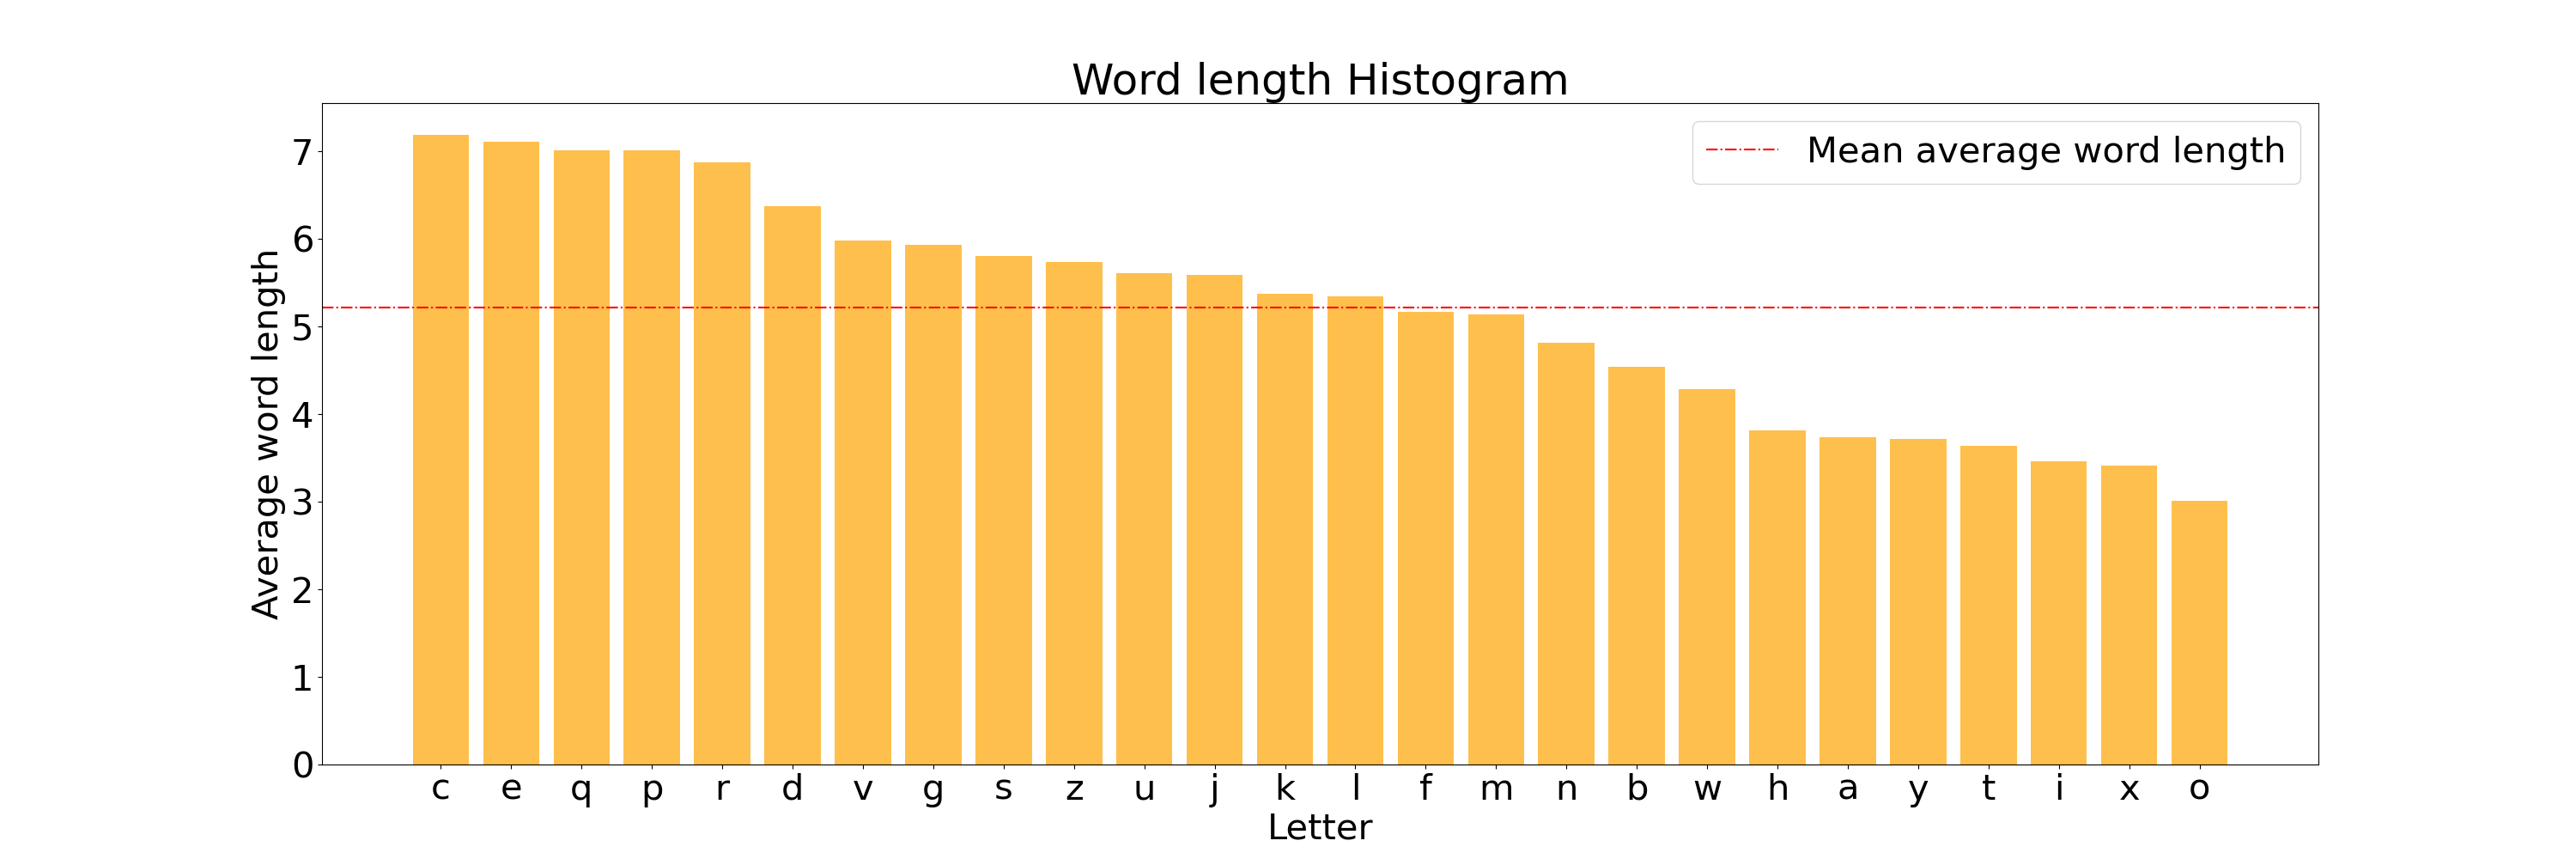
\includegraphics[width=\linewidth]{figures/download}
  \caption{A histogram depicting the average word length (y-axis) for every letter of the Latin alphabet (x-axis). The mean average length is shown as a horizontal red dashed line.}
  \label{img:histogram:word_lengths}
\end{figure}

\section{Problem 2: Movie Analytics}
\label{sec:problem2}
The second problem focuses on producing analytic insights from an IMDB dataset.


\subsection{Problem Statement}
Implement a \textbf{MapReduce} program to perform analytics tasks on an IMDB dataset about movies. The utter goal of your analysis would be to extract useful insights from the available movie data that will assist the IMDB team provide better recommendations for movies, based on their genre and/or country. In particular, the dataset (\texttt{movies.csv}) contains the following fields:
\begin{itemize}
  \item imdbID: unique identifier of the movie in the IMDB database
  \item title: the movie title
  \item year: the year the movie was first released
  \item duration: the duration of the movie
  \item genre(s): the genre or genres in which the movie is classified
  \item premier date: the date of the first showing of the movie
  \item score: the IMDB score of the movie
  \item country/-ies: the country or countries the movie was produced in
\end{itemize}

You are asked to implement Map-Reduce source code in Java programming language for the following analytics tasks:
\begin{itemize}
  \item Calculate the total duration of all movies per country. Note that in case multiple countries are recorded for a movie, the respective duration should be counted for all of them separately.
  \item Calculate the total number of movies per year and genre, having IMDB score over 8. For movies that have more than one genre, the sum should be separate for each genre.
\end{itemize}

\subsection{Proposed approach}
\subsubsection{Setting}
Our implementation is run and tested in a Linux environment with 12 cores, using the Java programming language.
We have used the Java Development Kit (JDK) version 11.0.11.
The source code is developed in IntelliJ IDEA Community Edition 2021.1.1 and managed using Maven as the build tool.

The project’s dependencies, including Hadoop libraries, are defined in the \texttt{pom.xml} file located in the root of
the repository.
The project is compiled and executed directly from IntelliJ IDEA.

To run the project, open the \texttt{MovieAnalyticsMaster} class in IntelliJ IDEA, and execute the main method.
You will need to specify the following command-line arguments:

\begin{itemize}
  \item \texttt{<input\_path>} specifies the directory containing the input text files, located at \texttt{map-reduce/movieAnalytics/ input}.
  \item \texttt{<output\_path>} specifies the directory where the MapReduce output will be written, which will be created in the \texttt{out} folder.
\end{itemize}

IntelliJ IDEA will handle the compilation and execution automatically when the main method is run. Make sure to configure the input and output paths as required for your specific run. Note that the command-line arguments must follow the specified order and format. If any of the arguments are missing or invalid, the program will terminate with an appropriate error message.

\subsubsection{Implementation}
The proposed approach leverages the MapReduce programming paradigm to compute the analytical insights for the two tasks. \autoref{img:movieAnalyticsSolutionDiagram} depicts the architecture of our solution as a diagram. We opt for executing two separate jobs; one for each task presented by the problem statement.

\begin{figure}[tb!]
  \centering
  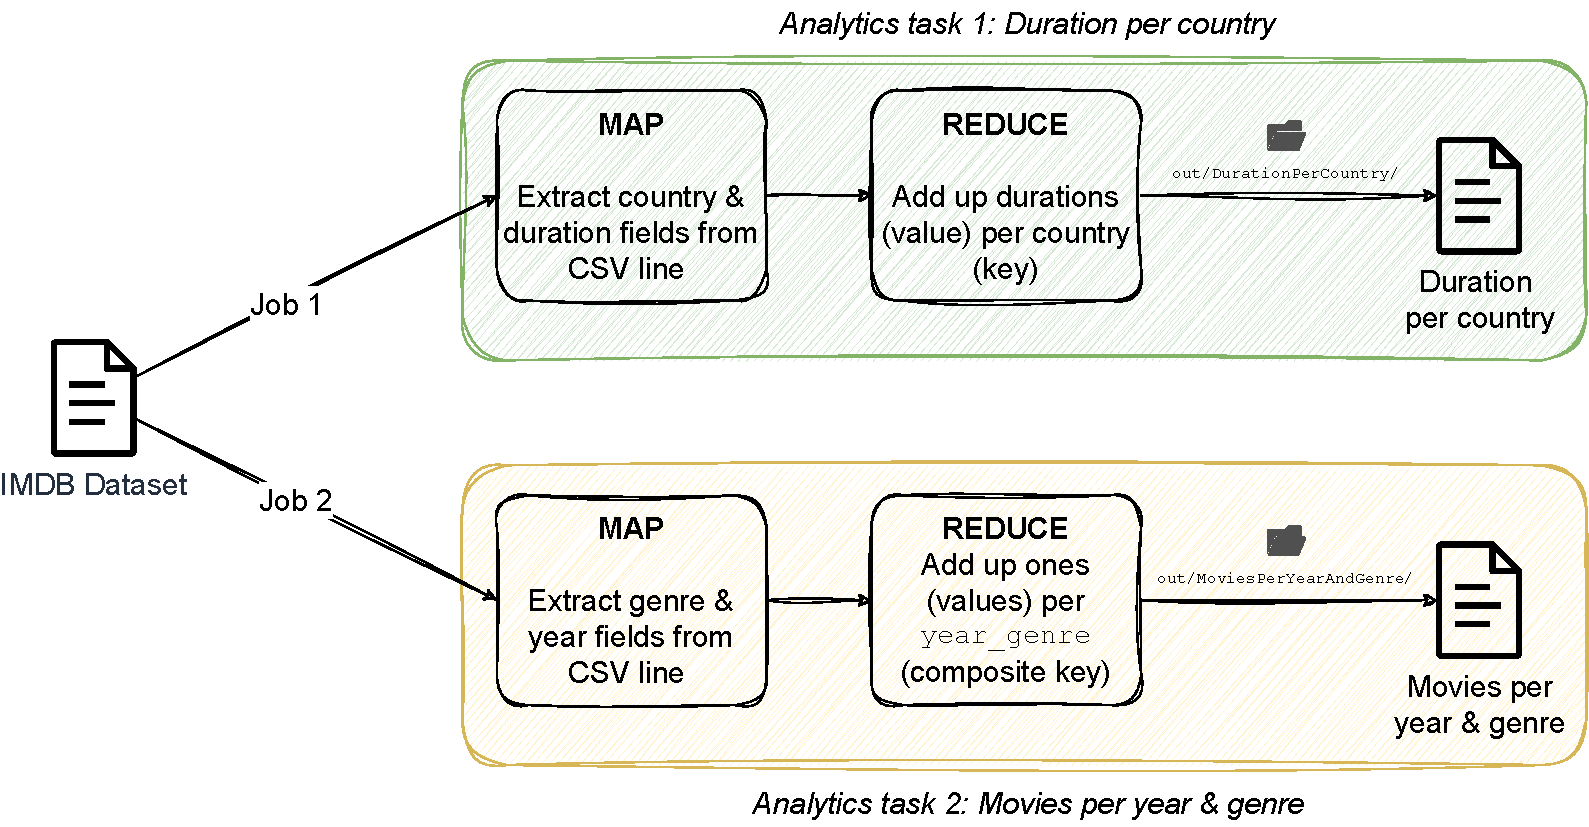
\includegraphics[width=0.8\linewidth]{figures/movieAnalytics}
  \caption{The MapReduce solution architecture for the movie analytics problem. Two separate jobs are executed to solve the two tasks, namely duration per country (green) and movies per year \& genre (yellow). The two tasks also create separate subdirectories for writing the results.}
  \label{img:movieAnalyticsSolutionDiagram}
\end{figure}

\paragraph{Task 1: Duration per country} One map-reduce cycle is enough to handle this task, as depicted in the top part of~\autoref{img:movieAnalyticsSolutionDiagram} in green color. The map function parses the CSV file line by line and extracts the useful fields from each line. In this case, the useful fields are the country (or countries) the movie was produced and the movie duration, i.e., the fourth and ninth fields in the input line respectively. We employ more complex logic to handle cases where there are multiple countries in a single movie. In particular, we parse again the field and tokenize it into the separate countries, producing a key-value pair for each country-duration pair within a movie. The reduce function is, then, trivial; it just adds up the durations (value) per country (key) and outputs the results. The interested reader can refer to the \texttt{CSVProcessor.java} (mapper), \texttt{AnayticsEngine.java} (reducer) and \texttt{MovieAnalyticsMaster.java} (driver) files for the source code implementation of our solution.

\paragraph{Task 2: Movies per year \& genre w.r.t. score constraint} The task is similar to the first one, with the only difference lying in the fields extracted from the input CSV line. In this case, we are interested about the year, the genre (or genres) and score fields, i.e., the third, fifth and seventh fields in the input CSV line. The map function produces key-value pairs in the form \texttt{(composite\_key, 1)}, where the composite key consists of the year and the genre of the respective movie concatenated by an underscore, e.g., \texttt{2024\_action}. We handle multiple genres per movie similarly with the multiple countries in task 1. We employ the same trivial reducer that adds up the values (ones) per (composite) key, as shown in the bottom part of~\autoref{img:movieAnalyticsSolutionDiagram} in yellow color.

\subsubsection{Evaluation} Our solution is tested using the provided IMDB dataset, namely \texttt{movies.csv}. We list the execution results in~\autoref{sec:data2}.

\section{Problem 3: Movie Analytics}
\label{sec:problem3}
The third problem focuses on producing analytic insights into a movies dataset.


\subsection{Problem Statement}
In this problem, you are provided with a dataset that contains information about movies. Each record represents a movie and includes three main columns (attributes), namely \texttt{movieId}, \texttt{title} and \texttt{genres}. An example record of the dataset is the following:

\begin{verbatim}
1,Toy Story (1995),Adventure|Animation|Children|Comedy|Fantasy
\end{verbatim}

Note that a movie can belong to multiple genres (e.g., adventure, fantasy, and so on). The genres are separated by a vertical line (`|') in the respective field. Your Apache Spark (Scala) application should compute the following analytics:
\begin{enumerate}
  \item \textbf{How many movies are there for each genre?} If a movie belongs to multiple genres, it should be counted to all these genres. Sort the results by the name of genre in alphabetical order.
  \item \textbf{How many movies have been filmed per year?} Note that the year a movie was filmed is currently encoded into a composite movie title, e.g., ``\texttt{Toy Story (1995)}''. Show the top 10 years with the most movies filmed within them.
  \item \textbf{Which are the words that appear at least 10 times in the titles of the movies, and what is their total frequency?} You can ignore words that have less than 4 characters. Sort the results, showing first the words with the higher frequency.
\end{enumerate}

\subsection{Proposed approach}
\subsubsection{Setting}
Our implementation is run and tested in a Linux environment with 12 cores, using the Scala programming language version 2.13.15 and Apache Spark version 3.5.3. We have used SBT as the build tool of our solution.
We have used the Software Development Kit (JDK) version 11.0.11.
The source code is developed in IntelliJ IDEA Community Edition 2021.1.1 and managed using SBT as the build tool. All dependencies of the project can be found in the \texttt{build.sbt} file located at the root folder of the project.
The project is compiled and executed directly from the IntelliJ IDEA.

To run the project, open the \texttt{src/main/scala/Task3MovieAnalytics.scala} file in IntelliJ IDEA, and execute the main method. After successful execution of the program, the results can be viewed under the \texttt{output/task3} directory.

\subsubsection{Implementation} We leverage Apache Spark \emph{DataFrames} API to calculate the aforementioned analytical queries. Our proposed approach comprises the following four stages:
\begin{description}
  \item[Stage 1:] Data cleaning and preprocessing
  \item[Stage 2:] Computation of genre analytics (query 1)
  \item[Stage 3:] Computation of year analytics (query 2)
  \item[Stage 4:] Computation of title analytics (query 3)
\end{description}
\autoref{img:movieAnalyticsSolutionDiagram} graphically depicts the four stages, as well as their assembly in a workflow. We elaborate on each stage separately in the rest of the Subsection.

\begin{figure}[tb!]
  \centering
  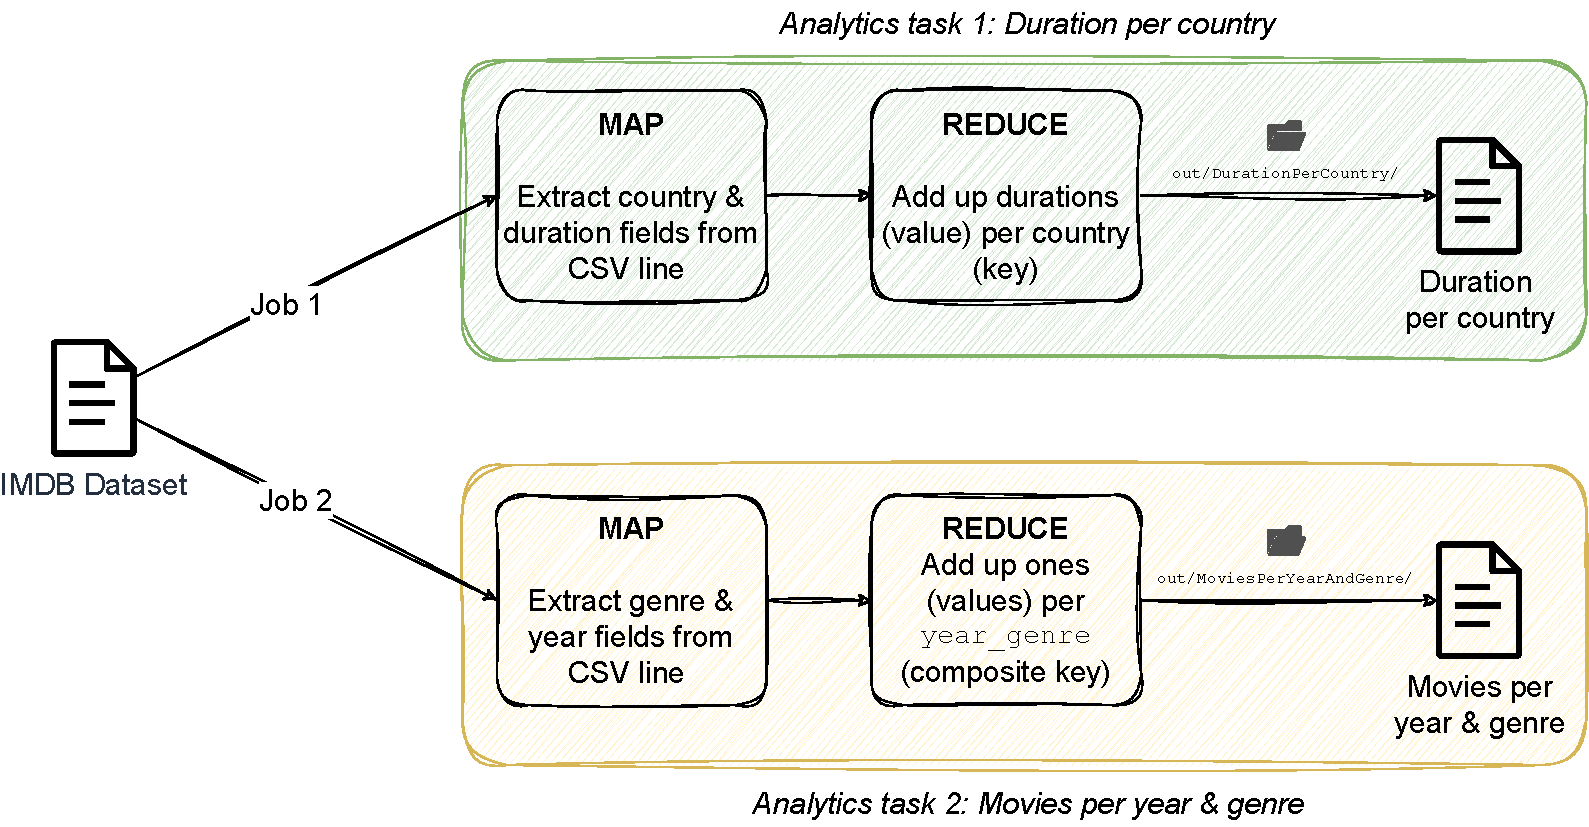
\includegraphics[width=0.7\linewidth]{figures/movieAnalytics}
  \caption{The MapReduce solution architecture for the movie analytics problem. Two separate jobs are executed to solve the two tasks, namely duration per country (green) and movies per year \& genre (yellow). The two tasks also create separate subdirectories for writing the results.}
  \label{img:movieAnalyticsSolutionDiagram}
\end{figure}

\paragraph{Stage1: Data Cleaning and preprocessing} In this stage, we address data quality issues that are present in the raw movie data. Missing production year, missing genres and trailing whitespaces in the title string are the detected data quality issues. To address these issues, we explicitly mark the movie year as ``N/A'' (not available) \& movie genre as ``(no genre listed)'' and trim the composite title strings, respectively. Subsequently, we transform the data representation to a more efficient form, by extracting the actual title and year to separate fields (instead of a composite one) and splitting the genres composite string field to an array of genres. Throughout the whole process, we \textbf{use solely the DataFrame API} of Apache Spark, leveraging also the pattern matching functionality of Scala. A small sample of the cleaned and transformed DataFrame shown in~\autoref{img:movieAnalyticsSolutionDiagram} is depicted below:

\begin{verbatim}
                  +-------+--------------------+--------------------+----+
                  |movieId|               title|              genres|year|
                  +-------+--------------------+--------------------+----+
                  |      1|           Toy Story|[Adventure, Anima...|1995|
                  |      2|             Jumanji|[Adventure, Child...|1995|
                  |      3|    Grumpier Old Men|   [Comedy, Romance]|1995|
                  |      4|   Waiting to Exhale|[Comedy, Drama, R...|1995|
                  |      5|Father of the Bri...|            [Comedy]|1995|
                  +-------+--------------------+--------------------+----+
\end{verbatim}

\paragraph{Stage 2: Computation of genre analytics} In this stage, we use the cleaned and transformed data to compute analytical insights into the movie genres. In particular, we use the DataFrame API (\texttt{select()}, \texttt{group\_by()}, etc.) to calculate the number of movies that belong to each genre. An implementation detail of our solution lies in handling the cases where a movie belongs to multiple genres. To ensure the integrity of the computed analytics, we opt for using the \texttt{explode()} function of the DataFrame API, to transform the array of genres to separate genre items. The analytics are, then, computed on top of this extra transformation, enabling us to include \textbf{a movie into the calculations of all the genres it belongs}.

\paragraph{Stage 3: Computation of year analytics} In this stage, we use the cleaned and transformed data to compute analytical insights into the movie production years. Similarly to Stage 2, we leverage exclusively the DataFrame API to calculate the total number of movies filmed each year. In this case, the \texttt{group\_by} operation is more straightforward, since the cleaned and transformed DataFrame contains a dedicated column for the movie production year.

\paragraph{Stage 4: Computation of title analytics} Similarly to Stage 2, we use operations available from the DataFrame API to calculate the most frequently used words in the movie titles. We, leverage the \texttt{split(" ")} and \texttt{explode()} functions to transform titles, first, into an array of words and, then, into separate words that are finally grouped and aggregated. We remove words that have less than 4 characters and fundamental stopwords, such as ``with'', or ``from'', in order to obtain analytical insights of high quality.

\subsubsection{Evaluation} Our solution is tested using the raw movie data, namely \texttt{movies.csv}. We list the execution results in~\autoref{sec:data3}.

\paragraph{Stage 2: Computation of genre analytics}
We list here the execution results for the genre analytics query in a 6-column format.
\begin{multicols}{6}
  \noindent
  Action: 7348
  \\ Adventure: 4145
  \\ Animation: 2929
  \\ Children: 2935
  \\ Comedy: 16870
  \\ Crime: 5319
  \\ Documentary: 5605
  \\ Drama: 25606
  \\ Fantasy: 2731
  \\ Film-Noir: 353
  \\ Horror: 5989
  \\ IMAX: 195
  \\ Musical: 1054
  \\ Mystery: 2925
  \\ Romance: 7719
  \\ Sci-Fi: 3595
  \\ Thriller: 8654
  \\ War: 1874
  \\ Western: 1399
  \\ N/A: 5062
\end{multicols}

\paragraph{Stage 3: Computation of year analytics}
We list here the execution results for the year analytics query in a 3-column format, i.e., the top 10 years with the most movies. We observe that these years span the time period between 2009 and 2018, excluding 2015, indicating a heavy film production process in this decade. \autoref{img:movies_per_year} depicts the distribution of movies per year for all years in chronological order. Our findings indicate a clear long-tail distribution of movies over the years, with a burst of new movies over the last decade.
\begin{multicols}{3}
  \centering
  \noindent
  2015: 2512 movies
  \\ 2016: 2488 movies
  \\ 2014: 2406 movies
  \\ 2017: 2373 movies
  \\ 2013: 2173 movies
  \\ 2018: 2032 movies
  \\ 2012: 1978 movies
  \\ 2011: 1838 movies
  \\ 2009: 1724 movies
  \\ 2010: 1691 movies
\end{multicols}

\begin{figure}[tb!]
  \centering
  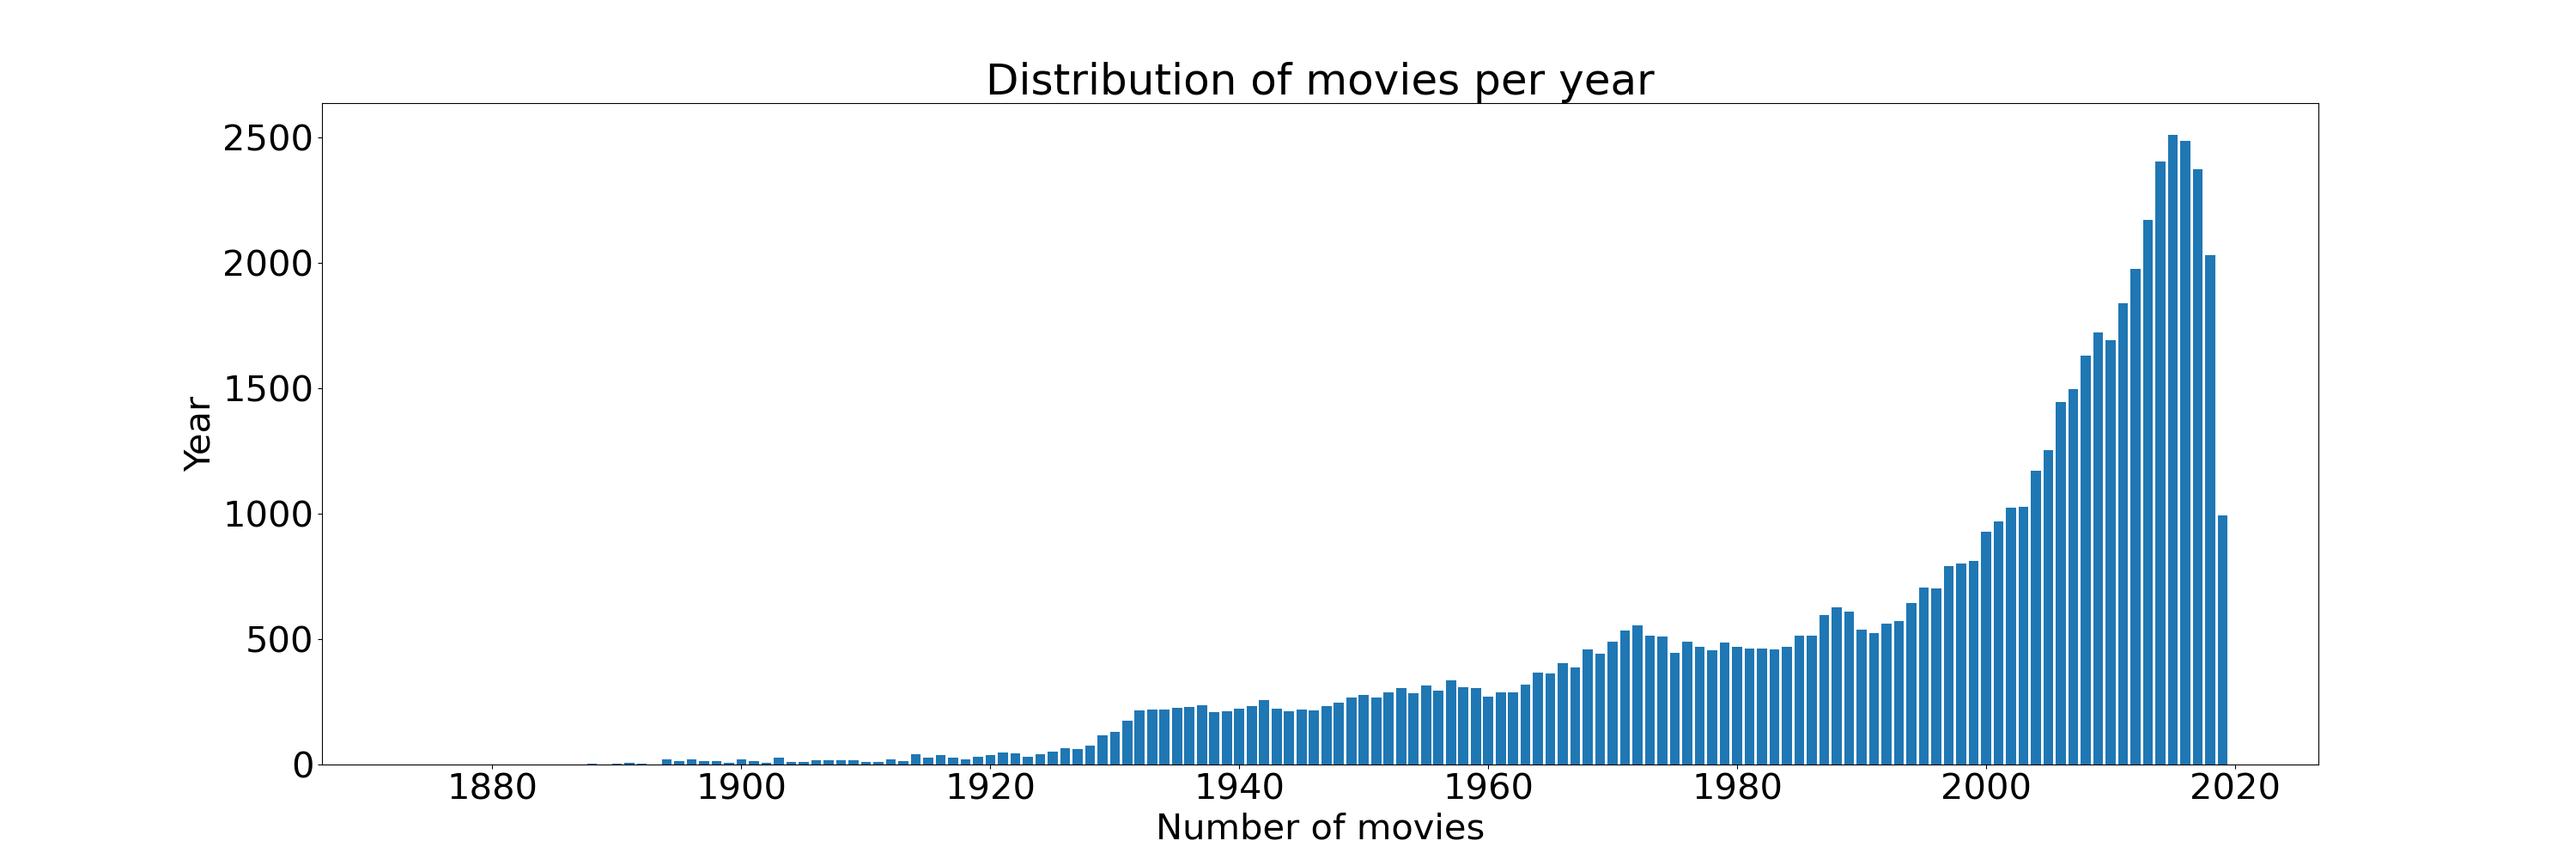
\includegraphics[width=\linewidth]{figures/movies per year}
  \caption{The distribution of the total number of movies per year in the dataset used for evaluating our solution.}
  \label{img:movies_per_year} 
\end{figure}

\paragraph{Stage 4: Computation of title analytics}
We list in~\autoref{sec:data3} the execution results for the title analytics query.Also, ~\autoref{img:word_cloud} depicts a word cloud with the most frequently used words in movie titles, found in the dataset used for evaluating our solution. Note that the bigger a word is, the more frequently it appears in movie titles.
\begin{figure}[tb!]
  \centering
  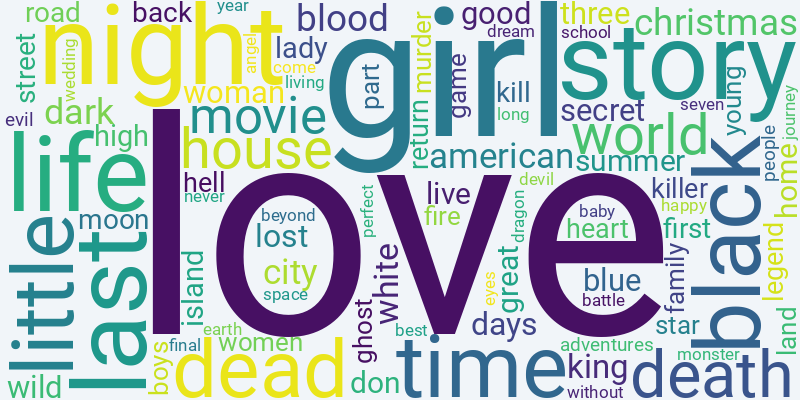
\includegraphics[width=0.8\linewidth]{figures/word cloud}
  \caption{A word cloud depicting the most frequent words appearing in the titles of the movies in the dataset examined. The bigger a word is, the more frequently it appears in the titles of the movies.}
  \label{img:word_cloud}
\end{figure}

\section{Problem 4: Probabilistic graph}
\label{sec:problem4}
We discuss here the fourth problem of the assignment.
The main target of the assignment is to get acquainted with performing various MapReduce phases on a pipeline frame.

\subsection{Problem Statement}
We are given an input file in text format where each line contains a connection between two vertices of a network and a
probability value.
For each edge \( e \), there is a probability value \( p(e) \) which indicates the probability that the two vertices are
connected by the edge.
Obviously, the values of \( p(e) \) range between 0 and 1.
The values in each line are separated by a space.
Consider the network shown in the previous figure.
The edge connecting vertices 4 and 5 has a probability of
0.8, the edge connecting vertices 2 and 3 has a probability of 0.2, etc.

\begin{figure}[h]
  \centering
  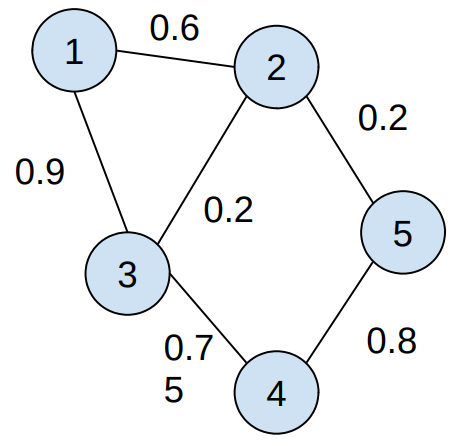
\includegraphics[width=0.25\linewidth]{figures/graph}
\end{figure}

The file corresponding to this graph would be:

\[
  1 \ 2 \ 0.6, \\
  1 \ 3 \ 0.9, \\
  2 \ 3 \ 0.2, \\
  3 \ 4 \ 0.75, \\
  2 \ 5 \ 0.2, \\
  4 \ 5 \ 0.8,
\]

The edges are generally stored in random order in the file, so we cannot assume they have a specific arrangement.

The following tasks are requested:

\begin{enumerate}
  \item Write a Java program that computes the average degree for all the vertices.
  \item The average degree is defined as the sum of the probabilities of the edges that fall on a vertex.
  \item For example, in the previous diagram, the average degree of vertex 3 is \( 0.9 + 0.2 + 0.75 = 1.85 \).
  \item Before performing this calculation, you should ignore all edges with a probability less than a threshold \( T \)
        , which should be passed as a parameter to the main function.
  \item Modify the code from task 1 so that, at the end, only the vertices with an average degree greater than the
        average of the degrees of all the vertices are displayed in the output.

\end{enumerate}

\subsection{Proposed approach}
\subsubsection{Setting}
Our implementation is run and tested in a Linux environment with 12 cores, using the Java programming language.
We have used the Java Development Kit (JDK) version 11.0.11.
The source code is developed in IntelliJ IDEA Community Edition 2021.1.1 and managed using Maven as the build tool.

The project’s dependencies, including Hadoop libraries, are defined in the \texttt{pom.xml} file located in the root of
the repository.
The project is compiled and executed directly from IntelliJ IDEA.

To run the project, open the \texttt{GraphMaster} class in IntelliJ IDEA, and execute the main method.
You will need to specify the following command-line arguments:

\begin{itemize}
  \item \texttt{<input\_path>} specifies the directory containing the input text files, located at
        \texttt{map-reduce/ probabilisticGraph /input}.
  \item \texttt{<output\_path>} specifies the directory where the MapReduce output will be written, which will be
        created in the \texttt{out} folder.
  \item \texttt{<T>} is the minimum edge-degree threshold for vertices to be included in the results.
\end{itemize}

IntelliJ IDEA will handle the compilation and execution automatically when the main method is run.
Make sure to configure the input and output paths as required for your specific run.

Note that the command-line arguments must follow the specified order and format.
If any of the arguments are missing or invalid, the program will terminate with an appropriate error message.

\subsubsection{Implementation}
The problem at hand involves processing a probabilistic graph, where each edge connects two vertices with a probability
value.
The task is to compute the average degree for each vertex, considering only edges whose probability exceeds a given
threshold \( T \).
The methodology proposed here utilizes a distributed MapReduce framework, implemented using Hadoop, to efficiently
process and analyze large-scale graph data.
The approach is divided into three main phases, each handled by separate MapReduce jobs, with intermediate results
passed between the phases.

The \texttt{GraphMaster} class serves as the orchestrator of the entire MapReduce process.
It manages the execution of the three phases, invoking the appropriate MapReduce jobs in sequence.
The main steps executed by \texttt{GraphMaster} are:

\begin{enumerate}
  \item It retrieves the command-line arguments, including the input and output directories as well as the threshold
        value \( T \), which determines which edges to consider in the graph.
  \item It initiates the first MapReduce job to compute the degree of each vertex in the graph.
        The input consists of edge data, and the output is a summation of edge probabilities for each vertex.
  \item After the first job completes, the \texttt{GraphMaster} starts the second MapReduce job to calculate the mean
        degree of the graph, using the results from the first job.
  \item Once the mean degree is computed, \texttt{GraphMaster} starts the third MapReduce job, which filters out the
        vertices with degrees lower than the mean degree.
  \item It cleans up intermediate directories after each phase and moves the final output to the desired location.
\end{enumerate}

\texttt{GraphMaster} coordinates these steps by configuring and executing the MapReduce jobs, ensuring that each phase
depends on the results of the previous one. \\

The entire process consists of three MapReduce jobs, executed sequentially:

\begin{enumerate}
  \item \textbf{Phase 1:} The first job computes the degree of each vertex by summing the probabilities of the edges
        connected to it.
        It produces intermediate results for each vertex.
  \item \textbf{Phase 2:} The second job calculates the mean degree by summing the degrees from the first phase and
        dividing by the total number of vertices.
  \item \textbf{Phase 3:} The third job filters out the vertices with a degree lower than the mean degree and produces
        the final filtered result.
\end{enumerate}

After each job completes, intermediate data is written to disk and passed as input to the subsequent job.
The final output consists of the vertices whose degree exceeds or equals the mean degree. \\

\textbf{Phase 1: Calculating Vertex Degree}
The first MapReduce job is responsible for calculating the degree of each vertex in the graph, where the degree is
defined as the sum of the probabilities of the edges connected to that vertex.
The degree of each vertex is computed by the \texttt{GraphMapper} and \texttt{GraphReducer} classes.

The \texttt{GraphMapper} class reads each edge from the input data, which consists of lines containing two vertices
and the associated probability value.
It splits each line into two components (the two vertices), and for each vertex, it emits the corresponding probability
value as the output.
The mapper also checks if the probability value exceeds the threshold \( T \), which is provided as a configuration
parameter.
If the probability is greater than or equal to \( T \), it emits the vertex along with the corresponding probability.

The \texttt{GraphReducer} class receives the vertex and associated probability values emitted by the mapper.
For each vertex, it sums up all the probabilities of the edges connected to that vertex, and emits the pair as output.

\textbf{Phase 2: Calculating the Mean Degree}
The second phase of the approach calculates the mean degree of all vertices.
This is done by summing the degree values from the previous phase and dividing by the total number of vertices.

The \texttt{MeanMapper} class receives the degree values from the output of the first MapReduce job.
It emits two key-value pairs for each input line: a count of the number of vertices and the sum of the degree values.
These are emitted with fixed keys (\texttt{"count"} and \texttt{"sum"}) so that they can be aggregated in the reducer.

The \texttt{MeanReducer} class processes the count and sum values emitted by the mapper.
It calculates the total sum and count of vertices and then writes these values as output.
The mean degree is calculated by dividing the sum by the count, and the result is stored for use in the next phase.

\textbf{Phase 3: Filtering Vertices by Mean Degree}
In the third phase, the vertices whose degree is greater than or equal to the mean degree calculated in Phase 2 are
selected.
This phase uses the results from Phase 1 and Phase 2, applying the filtering criteria to retain only those vertices with
a degree greater than or equal to the mean.

The \texttt{FilterMapper} class takes the degree values emitted by the first reducer and writes them as key-value pairs.
Each key is a vertex, and the value is the degree of that vertex.
The mapper does not perform any filtering; instead, it simply passes the values along to the reducer.

The \texttt{FilterReducer} class filters out the vertices whose degree is less than the mean degree.
It retrieves the mean degree from the configuration, and for each vertex, it compares the degree value to the mean.
If the degree is greater than or equal to the mean, it emits the vertex along with its degree.
This final output contains only the vertices that satisfy the filtering criteria.

\subsubsection{Evaluation}
The experiments were executed using the dataset `collins.txt` with a parameter setting of \( T = 0.8 \).

To provide a comprehensive overview, the results of the experiment, including the detailed values derived from the
dataset, are presented in~\autoref{sec:data4} in a 2-column format.



\section{Conclusion}
\label{sec:conclusion}
In this document we have presented our solutions and rationale for solving the second assignment of the M.Sc.
course on \emph{Technologies for Big Data Analysis}, offered by the \emph{DWS M.Sc. Program}. For each one of the four problems of the assignment, we have presented their statement, as well as the solution approach we have adopted. All execution results with the provided datasets can be found in the appendices of our work.

\newpage
\appendix

\section{Problem 2 execution results}
\label{sec:data2}
We list here the execution results of our solution for the second problem (movie analytics) tested on the \texttt{movies.csv} dataset. Task 1 (duration per country) produces the following results:

\begin{multicols}{4}
  \noindent
  Afghanistan:	815
  \\ Albania:	646
  \\ Algeria:	2115
  \\ American Samoa:	247
  \\ Angola:	357
  \\ Argentina:	28813
  \\ Armenia:	264
  \\ Aruba:	739
  \\ Australia:	66068
  \\ Austria:	22925
  \\ Bahamas:	560
  \\ Bahrain:	87
  \\ Bangladesh:	429
  \\ Barbados:	92
  \\ Belarus:	427
  \\ Belgium:	54192
  \\ Bermuda:	95
  \\ Bhutan:	291
  \\ Bolivia:	797
  \\ Bosnia and Herzegovina:	2207
  \\ Botswana:	295
  \\ Brazil:	27333
  \\ Bulgaria:	5430
  \\ Burkina Faso:	903
  \\ Burma:	95
  \\ Cambodia:	894
  \\ Cameroon:	615
  \\ Canada:	210826
  \\ Chad:	493
  \\ Chile:	6178
  \\ China:	42089
  \\ Colombia:	3810
  \\ Congo:	88
  \\ Costa Rica:	431
  \\ Croatia:	4340
  \\ Cuba:	2899
  \\ Cyprus:	948
  \\ Czech Republic:	15317
  \\ Czechoslovakia:	8434
  \\ C\'ote d'Ivoire:	180
  \\ Denmark:	44186
  \\ Dominican Republic:	866
  \\ East Germany:	2095
  \\ Ecuador:	893
  \\ Egypt:	3090
  \\ El Salvador:	167
  \\ Estonia:	4651
  \\ Ethiopia:	537
  \\ Faroe Islands:	97
  \\ Federal Republic of Yugoslavia:	2167
  \\ Finland:	48990
  \\ France:	467279
  \\ Gabon:	80
  \\ Georgia:	1846
  \\ Germany:	226808
  \\ Ghana:	655
  \\ Greece:	20305
  \\ Greenland:	90
  \\ Grenada:	79
  \\ Guatemala:	638
  \\ Guinea:	90
  \\ Haiti:	498
  \\ Honduras:	80
  \\ Hong Kong:	66567
  \\ Hungary:	19668
  \\ Iceland:	7839
  \\ India:	110215
  \\ Indonesia:	3931
  \\ Iran:	11762
  \\ Iraq:	1365
  \\ Ireland:	26506
  \\ Isle Of Man:	396
  \\ Israel:	16662
  \\ Italy:	288407
  \\ Jamaica:	807
  \\ Japan:	178558
  \\ Jordan:	1313
  \\ Kazakhstan:	2145
  \\ Kenya:	523
  \\ Korea:	90
  \\ Kosovo:	188
  \\ Kuwait:	273
  \\ Kyrgyzstan:	400
  \\ Laos:	289
  \\ Latvia:	2297
  \\ Lebanon:	1289
  \\ Liberia:	283
  \\ Libya:	520
  \\ Liechtenstein:	1011
  \\ Lithuania:	3772
  \\ Luxembourg:	11976
  \\ Macao:	175
  \\ Madagascar:	204
  \\ Malaysia:	1338
  \\ Mali:	220
  \\ Malta:	885
  \\ Martinique:	103
  \\ Mauritania:	515
  \\ Mexico:	35560
  \\ Micronesia:	85
  \\ Moldova:	95
  \\ Monaco:	189
  \\ Mongolia:	186
  \\ Montenegro:	439
  \\ Morocco:	4525
  \\ Namibia:	105
  \\ Nepal:	797
  \\ Netherlands:	47054
  \\ New Zealand:	14561
  \\ Nicaragua:	183
  \\ Nigeria:	494
  \\ North Korea:	508
  \\ Norway:	26476
  \\ Pakistan:	1728
  \\ Palestine:	1530
  \\ Panama:	903
  \\ Papua New Guinea:	295
  \\ Paraguay:	317
  \\ Peru:	2436
  \\ Philippines:	7882
  \\ Poland:	35543
  \\ Portugal:	15232
  \\ Puerto Rico:	1322
  \\ Qatar:	1036
  \\ Republic of Macedonia:	1515
  \\ Reunion:	38
  \\ Romania:	15739
  \\ Russia:	50757
  \\ Rwanda:	527
  \\ Samoa:	110
  \\ Saudi Arabia:	490
  \\ Senegal:	1462
  \\ Serbia:	4337
  \\ Serbia and Montenegro:	1314
  \\ Singapore:	4557
  \\ Slovakia:	2525
  \\ Slovenia:	2956
  \\ Somalia:	90
  \\ South Africa:	14688
  \\ South Korea:	56245
  \\ Soviet Union:	51353
  \\ Spain:	116651
  \\ Sri Lanka:	318
  \\ Suriname:	105
  \\ Sweden:	68956
  \\ Switzerland:	34516
  \\ Syria:	447
  \\ Taiwan:	16618
  \\ Tajikistan:	351
  \\ Tanzania:	441
  \\ Thailand:	10189
  \\ The Democratic Republic Of Congo:	98
  \\ Trinidad and Tobago:	86
  \\ Tunisia:	2236
  \\ Turkey:	20068
  \\ UK:	492616
  \\ USA:	2276142
  \\ Uganda:	243
  \\ Ukraine:	4616
  \\ United Arab Emirates:	3202
  \\ Uruguay:	2038
  \\ Uzbekistan:	324
  \\ Vanuatu:	100
  \\ Venezuela:	2014
  \\ Vietnam:	1261
  \\ West Germany:	58480
  \\ Yugoslavia:	8742
  \\ Zaire:	80
  \\ Zimbabwe:	210
\end{multicols}

Task 2 (movies per year and genre) produces the following results:

\begin{multicols}{4}
  \noindent
  1973\_Adventure:	1
  \\ 1973\_Drama:	1
  \\ 1973\_History:	1
  \\ 1976\_Comedy:	2
  \\ 1976\_Drama:	1
  \\ 1976\_History:	1
  \\ 1976\_Mystery:	1
  \\ 1976\_Romance:	1
  \\ 1979\_Adventure:	1
  \\ 1979\_Crime:	1
  \\ 1979\_Mystery:	1
  \\ 1982\_Comedy:	1
  \\ 1982\_Drama:	1
  \\ 1985\_Documentary:	1
  \\ 1985\_History:	1
  \\ 1988\_Comedy:	1
  \\ 1988\_Drama:	2
  \\ 1988\_Sci-Fi:	1
  \\ 1996\_Documentary:	1
  \\ 1996\_Music:	1
  \\ 2001\_Documentary:	1
  \\ 2001\_Music:	1
  \\ 2002\_Documentary:	1
  \\ 2002\_Music:	1
  \\ 2004\_Adventure:	1
  \\ 2004\_Documentary:	2
  \\ 2004\_Drama:	1
  \\ 2004\_Music:	1
  \\ 2004\_Romance:	1
  \\ 2006\_Animation:	1
  \\ 2006\_Crime:	1
  \\ 2006\_Drama:	1
  \\ 2007\_Documentary:	1
  \\ 2007\_War:	1
  \\ 2008\_Action:	1
  \\ 2008\_Crime:	1
  \\ 2008\_Drama:	1
  \\ 2009\_Documentary:	1
  \\ 2015\_Action:	1
  \\ 2015\_Adventure:	1
  \\ 2015\_Animation:	1
  \label{multicol:test}
\end{multicols}

\section{Problem 3 execution results}
\label{sec:data3}
\begin{multicols}{6}
  % \centering
  \noindent
  love: 851
  \\ night: 519
  \\ story: 495
  \\ life: 476
  \\ last: 451
  \\ girl: 387
  \\ black: 352
  \\ time: 350
  \\ little: 335
  \\ dead: 327
  \\ death: 323
  \\ house: 311
  \\ world: 306
  \\ movie: 286
  \\ christmas: 274
  \\ blood: 271
  \\ dark: 258
  \\ city: 250
  \\ american: 249
  \\ white: 235
  \\ your: 225
  \\ king: 219
  \\ lost: 209
  \\ days: 209
  \\ secret: 202
  \\ that: 201
  \\ blue: 200
  \\ woman: 197
  \\ good: 196
  \\ three: 194
  \\ wild: 192
  \\ summer: 185
  \\ great: 181
  \\ home: 181
  \\ girls: 180
  \\ don't: 179
  \\ live: 179
  \\ lady: 169
  \\ island: 168
  \\ high: 166
  \\ this: 165
  \\ road: 159
  \\ back: 158
  \\ what: 156
  \\ kill: 156
  \\ street: 155
  \\ moon: 154
  \\ first: 153
  \\ about: 152
  \\ the): 147
  \\ hell: 146
  \\ legend: 146
  \\ killer: 145
  \\ heart: 145
  \\ return: 144
  \\ when: 142
  \\ like: 142
  \\ young: 139
  \\ ghost: 138
  \\ family: 137
  \\ star: 137
  \\ women: 135
  \\ part: 135
  \\ boys: 134
  \\ game: 133
  \\ murder: 129
  \\ land: 129
  \\ fire: 125
  \\ adventures: 121
  \\ people: 121
  \\ under: 120
  \\ after: 117
  \\ evil: 116
  \\ down: 114
  \\ journey: 114
  \\ never: 114
  \\ beyond: 113
  \\ devil: 112
  \\ perfect: 111
  \\ living: 111
  \\ long: 110
  \\ space: 108
  \\ monster: 108
  \\ wedding: 108
  \\ school: 108
  \\ best: 108
  \\ year: 107
  \\ battle: 106
  \\ final: 106
  \\ baby: 106
  \\ come: 106
  \\ angel: 105
  \\ eyes: 104
  \\ happy: 103
  \\ before: 102
  \\ earth: 101
  \\ without: 101
  \\ dragon: 101
  \\ dream: 101
  \\ seven: 100
  \\ kiss: 99
  \\ room: 99
  \\ magic: 99
  \\ it's: 98
  \\ party: 98
  \\ just: 98
  \\ town: 98
  \\ children: 98
  \\ man,: 98
  \\ will: 97
  \\ four: 97
  \\ tale: 97
  \\ heaven: 97
  \\ other: 95
  \\ river: 95
  \\ fear: 95
  \\ over: 95
  \\ they: 94
  \\ here: 94
  \\ golden: 93
  \\ sweet: 93
  \\ five: 93
  \\ years: 92
  \\ beautiful: 92
  \\ film: 91
  \\ west: 91
  \\ case: 91
  \\ green: 90
  \\ crazy: 88
  \\ water: 88
  \\ once: 88
  \\ fall: 87
  \\ song: 87
  \\ wolf: 86
  \\ paris: 85
  \\ deadly: 85
  \\ queen: 85
  \\ america: 84
  \\ miss: 84
  \\ true: 84
  \\ midnight: 84
  \\ into: 83
  \\ hero: 83
  \\ snow: 82
  \\ dance: 81
  \\ light: 81
  \\ jack: 81
  \\ hard: 81
  \\ goes: 81
  \\ hollywood: 80
  \\ only: 79
  \\ princess: 79
  \\ rock: 79
  \\ another: 79
  \\ dreams: 78
  \\ prince: 78
  \\ angels: 78
  \\ john: 77
  \\ escape: 77
  \\ terror: 77
  \\ cold: 77
  \\ shadow: 77
  \\ zero: 76
  \\ brothers: 76
  \\ call: 76
  \\ strange: 76
  \\ take: 75
  \\ inside: 75
  \\ money: 74
  \\ iron: 74
  \\ charlie: 74
  \\ country: 74
  \\ wind: 74
  \\ side: 74
  \\ wife: 73
  \\ mystery: 73
  \\ paradise: 73
  \\ tales: 73
  \\ where: 73
  \\ bride: 73
  \\ father: 72
  \\ again: 72
  \\ gold: 72
  \\ mountain: 71
  \\ truth: 71
  \\ revenge: 71
  \\ book: 71
  \\ beast: 69
  \\ face: 69
  \\ lucky: 69
  \\ adventure: 69
  \\ edge: 69
  \\ york: 69
  \\ deep: 69
  \\ hotel: 68
  \\ devil's: 68
  \\ vampire: 68
  \\ stranger: 68
  \\ dawn: 68
  \\ child: 68
  \\ behind: 68
  \\ name: 67
  \\ mother: 67
  \\ dangerous: 67
  \\ planet: 67
  \\ trouble: 67
  \\ born: 67
  \\ crime: 66
  \\ special: 66
  \\ there: 66
  \\ winter: 66
  \\ park: 66
  \\ blues: 66
  \\ human: 66
  \\ lives: 66
  \\ lake: 66
  \\ meet: 66
  \\ north: 66
  \\ friends: 65
  \\ beach: 65
  \\ silent: 65
  \\ free: 65
  \\ next: 65
  \\ times: 65
  \\ captain: 65
  \\ have: 65
  \\ jungle: 65
  \\ tomorrow: 64
  \\ forever: 64
  \\ dirty: 64
  \\ detective: 64
  \\ away: 64
  \\ curse: 64
  \\ alien: 64
  \\ body: 63
  \\ train: 63
  \\ double: 63
  \\ private: 63
  \\ second: 63
  \\ alone: 63
  \\ darkness: 63
  \\ daughter: 62
  \\ diary: 62
  \\ nothing: 62
  \\ point: 62
  \\ beauty: 61
  \\ spring: 61
  \\ history: 61
  \\ broken: 61
  \\ were: 61
  \\ play: 61
  \\ nightmare: 60
  \\ comedy: 60
  \\ comes: 59
  \\ master: 59
  \\ place: 59
  \\ naked: 58
  \\ super: 58
  \\ johnny: 58
  \\ made: 58
  \\ killing: 58
  \\ show: 57
  \\ stars: 57
  \\ (les: 57
  \\ witch: 57
  \\ santa: 57
  \\ holiday: 57
  \\ rose: 57
  \\ still: 56
  \\ nights: 56
  \\ ride: 56
  \\ hill: 56
  \\ things: 56
  \\ flight: 56
  \\ upon: 56
  \\ fury: 56
  \\ rise: 55
  \\ rain: 55
  \\ garden: 55
  \\ club: 55
  \\ brother: 55
  \\ right: 55
  \\ know: 55
  \\ doctor: 55
  \\ valley: 54
  \\ phantom: 54
  \\ treasure: 54
  \\ machine: 54
  \\ zombie: 54
  \\ blind: 54
  \\ glory: 54
  \\ force: 54
  \\ horse: 53
  \\ power: 53
  \\ welcome: 53
  \\ castle: 53
  \\ head: 53
  \\ music: 53
  \\ massacre: 52
  \\ attack: 52
  \\ real: 52
  \\ camp: 52
  \\ going: 52
  \\ fight: 52
  \\ kids: 52
  \\ shadows: 52
  \\ affair: 52
  \\ miracle: 51
  \\ hunter: 51
  \\ flying: 51
  \\ soul: 51
  \\ small: 51
  \\ alive: 51
  \\ future: 50
  \\ heroes: 50
  \\ london: 50
  \\ dogs: 50
  \\ through: 50
  \\ something: 50
  \\ vengeance: 50
  \\ tiger: 50
  \\ operation: 49
  \\ more: 49
  \\ wars: 49
  \\ sunday: 49
  \\ mary: 49
  \\ flesh: 49
  \\ between: 49
  \\ gang: 49
  \\ secrets: 49
  \\ broadway: 49
  \\ china: 49
  \\ skin: 48
  \\ love,: 48
  \\ stone: 48
  \\ grace: 48
  \\ horror: 48
  \\ iii:: 48
  \\ invisible: 48
  \\ storm: 48
  \\ walk: 48
  \\ sword: 48
  \\ line: 48
  \\ mind: 48
  \\ friend: 47
  \\ mrs.: 47
  \\ samurai: 47
  \\ you're: 47
  \\ bill: 47
  \\ express: 47
  \\ against: 47
  \\ most: 47
  \\ came: 47
  \\ harry: 46
  \\ texas: 46
  \\ enemy: 46
  \\ hunt: 46
  \\ silence: 46
  \\ hearts: 46
  \\ ninja: 46
  \\ george: 46
  \\ company: 46
  \\ open: 46
  \\ stories: 46
  \\ haunted: 45
  \\ full: 45
  \\ desert: 45
  \\ lies: 44
  \\ tokyo: 44
  \\ always: 44
  \\ door: 44
  \\ mine: 44
  \\ les): 44
  \\ left: 44
  \\ project: 44
  \\ glass: 44
  \\ lovers: 44
  \\ make: 44
  \\ dear: 44
  \\ hour: 44
  \\ hands: 44
  \\ gone: 44
  \\ soldier: 44
  \\ very: 44
  \\ sister: 44
  \\ hope: 43
  \\ voyage: 43
  \\ david: 43
  \\ hidden: 43
  \\ alice: 43
  \\ dust: 43
  \\ grand: 43
  \\ louis: 43
  \\ demon: 43
  \\ missing: 43
  \\ mission: 43
  \\ rising: 43
  \\ guns: 43
  \\ state: 43
  \\ being: 43
  \\ romance: 43
  \\ making: 43
  \\ called: 43
  \\ trail: 42
  \\ wall: 42
  \\ thief: 42
  \\ code: 42
  \\ yellow: 42
  \\ tell: 42
  \\ than: 42
  \\ tree: 42
  \\ thing: 42
  \\ pink: 42
  \\ sisters: 42
  \\ holy: 42
  \\ story,: 42
  \\ sleep: 42
  \\ bloody: 42
  \\ killed: 42
  \\ can't: 41
  \\ forbidden: 41
  \\ bridge: 41
  \\ mars: 41
  \\ chapter: 41
  \\ morning: 41
  \\ class: 41
  \\ michael: 41
  \\ breaking: 41
  \\ warrior: 41
  \\ goodbye: 41
  \\ justice: 41
  \\ frankenstein: 41
  \\ kingdom: 40
  \\ faces: 40
  \\ touch: 40
  \\ heat: 40
  \\ anna: 40
  \\ fast: 40
  \\ kung: 40
  \\ late: 40
  \\ games: 40
  \\ teenage: 40
  \\ work: 40
  \\ dracula: 40
  \\ freedom: 40
  \\ vacation: 40
  \\ man's: 40
  \\ trip: 40
  \\ cool: 40
  \\ i'll: 39
  \\ must: 39
  \\ everything: 39
  \\ brave: 39
  \\ kind: 39
  \\ giant: 39
  \\ shark: 39
  \\ third: 39
  \\ want: 39
  \\ sound: 39
  \\ bird: 39
  \\ confessions: 39
  \\ honor: 39
  \\ monsters: 39
  \\ business: 39
  \\ fish: 39
  \\ lion: 38
  \\ passion: 38
  \\ portrait: 38
  \\ wrong: 38
  \\ youth: 38
  \\ across: 38
  \\ million: 38
  \\ every: 38
  \\ look: 38
  \\ chance: 38
  \\ running: 38
  \\ flower: 37
  \\ burning: 37
  \\ unknown: 37
  \\ savage: 37
  \\ bear: 37
  \\ date: 37
  \\ let's: 37
  \\ fever: 37
  \\ search: 37
  \\ forest: 37
  \\ sherlock: 37
  \\ life,: 37
  \\ funny: 37
  \\ pretty: 37
  \\ ever: 37
  \\ circle: 36
  \\ saint: 36
  \\ thunder: 36
  \\ revolution: 36
  \\ takes: 36
  \\ race: 36
  \\ cinderella: 36
  \\ minutes: 36
  \\ national: 36
  \\ police: 36
  \\ coming: 36
  \\ hours: 36
  \\ friday: 36
  \\ better: 36
  \\ walking: 36
  \\ gods: 36
  \\ lone: 36
  \\ wonderful: 36
  \\ brain: 36
  \\ thousand: 36
  \\ army: 35
  \\ above: 35
  \\ french: 35
  \\ royal: 35
  \\ wish: 35
  \\ jane: 35
  \\ short: 35
  \\ century: 35
  \\ quiet: 35
  \\ south: 35
  \\ within: 34
  \\ greatest: 34
  \\ agent: 34
  \\ hand: 34
  \\ woman,: 34
  \\ kings: 34
  \\ central: 34
  \\ beginning: 34
  \\ zombies: 34
  \\ season: 34
  \\ ghosts: 34
  \\ rage: 34
  \\ frank: 34
  \\ empire: 34
  \\ happiness: 34
  \\ billy: 34
  \\ hood: 34
  \\ easy: 34
  \\ legacy: 34
  \\ east: 34
  \\ half: 34
  \\ weekend: 34
  \\ bullet: 34
  \\ among: 33
  \\ blonde: 33
  \\ chasing: 33
  \\ spirit: 33
  \\ amazing: 33
  \\ hate: 33
  \\ silver: 33
  \\ married: 33
  \\ bang: 33
  \\ shoot: 33
  \\ souls: 33
  \\ around: 33
  \\ worlds: 33
  \\ shot: 33
  \\ number: 33
  \\ blade: 32
  \\ trial: 32
  \\ robin: 32
  \\ their: 32
  \\ madness: 32
  \\ ring: 32
  \\ paul: 32
  \\ richard: 32
  \\ looking: 32
  \\ lord: 32
  \\ carry: 32
  \\ beat: 32
  \\ some: 31
  \\ henry: 31
  \\ untold: 31
  \\ stand: 31
  \\ action: 31
  \\ berlin: 31
  \\ past: 31
  \\ tour: 31
  \\ lover: 31
  \\ wonder: 31
  \\ generation: 31
  \\ jesus: 31
  \\ them: 31
  \\ talk: 31
  \\ woods: 31
  \\ monkey: 31
  \\ brown: 31
  \\ movie:: 31
  \\ jimmy: 31
  \\ wanted: 31
  \\ strangers: 30
  \\ honey: 30
  \\ butterfly: 30
  \\ eagle: 30
  \\ marriage: 30
  \\ falling: 30
  \\ hills: 30
  \\ letter: 30
  \\ steel: 30
  \\ killers: 30
  \\ scooby-doo!: 30
  \\ perry: 30
  \\ wings: 30
  \\ public: 30
  \\ warriors: 30
  \\ break: 30
  \\ snake: 30
  \\ mark: 30
  \\ color: 30
  \\ dancing: 30
  \\ tears: 30
  \\ danger: 30
  \\ county: 30
  \\ lonely: 30
  \\ elephant: 30
  \\ keep: 30
  \\ almost: 30
  \\ flowers: 29
  \\ quest: 29
  \\ returns: 29
  \\ movie,: 29
  \\ meets: 29
  \\ guys: 29
  \\ circus: 29
  \\ manhattan: 29
  \\ world,: 29
  \\ sing: 29
  \\ nowhere: 29
  \\ band: 29
  \\ beneath: 29
  \\ remember: 29
  \\ finding: 29
  \\ rabbit: 29
  \\ musical: 29
  \\ lights: 29
  \\ nine: 29
  \\ getting: 29
  \\ picture: 29
  \\ gangster: 29
  \\ loves: 29
  \\ farm: 28
  \\ magnificent: 28
  \\ sleeping: 28
  \\ below: 28
  \\ chan: 28
  \\ happened: 28
  \\ belle: 28
  \\ roll: 28
  \\ merry: 28
  \\ doll: 28
  \\ ball: 28
  \\ you,: 28
  \\ chinese: 28
  \\ grave: 28
  \\ zone: 28
  \\ rome: 28
  \\ creek: 28
  \\ brooklyn: 28
  \\ wonderland: 28
  \\ waiting: 28
  \\ pirates: 28
  \\ della: 28
  \\ cinema: 28
  \\ jones: 28
  \\ those: 27
  \\ hercules: 27
  \\ falls: 27
  \\ holmes: 27
  \\ scream: 27
  \\ uncle: 27
  \\ assassin: 27
  \\ luck: 27
  \\ adam: 27
  \\ fine: 27
  \\ seventh: 27
  \\ border: 27
  \\ female: 27
  \\ team: 27
  \\ playing: 27
  \\ dollar: 27
  \\ control: 27
  \\ barbie: 27
  \\ duck: 27
  \\ sons: 27
  \\ birds: 27
  \\ violence: 27
  \\ till: 27
  \\ order: 27
  \\ moment: 27
  \\ halloween: 27
  \\ village: 27
  \\ change: 27
  \\ werewolf: 27
  \\ witness: 27
  \\ give: 27
  \\ ladies: 27
  \\ apocalypse: 27
  \\ (zatôichi: 27
  \\ stop: 27
  \\ watch: 26
  \\ bunny: 26
  \\ rich: 26
  \\ peter: 26
  \\ haunting: 26
  \\ tarzan: 26
  \\ jeff: 26
  \\ sunshine: 26
  \\ please: 26
  \\ highway: 26
  \\ radio: 26
  \\ (die: 26
  \\ these: 26
  \\ dinner: 26
  \\ student: 26
  \\ dick: 26
  \\ august: 26
  \\ tall: 26
  \\ virgin: 26
  \\ mask: 26
  \\ voice: 26
  \\ price: 26
  \\ step: 26
  \\ fist: 26
  \\ bachelor: 26
  \\ violent: 26
  \\ eden: 26
  \\ demons: 26
  \\ burn: 25
  \\ satan: 25
  \\ mason:: 25
  \\ batman: 25
  \\ conspiracy: 25
  \\ rainbow: 25
  \\ ballad: 25
  \\ wicked: 25
  \\ harvest: 25
  \\ loved: 25
  \\ streets: 25
  \\ autumn: 25
  \\ match: 25
  \\ nation: 25
  \\ fighting: 25
  \\ together: 25
  \\ april: 25
  \\ madame: 25
  \\ taxi: 25
  \\ psycho: 25
  \\ damned: 25
  \\ bell: 25
  \\ nobody: 25
  \\ scarlet: 25
  \\ fatal: 25
  \\ cross: 25
  \\ cowboy: 25
  \\ resurrection: 25
  \\ animals: 25
  \\ shaolin: 25
  \\ memory: 25
  \\ twilight: 25
  \\ wolves: 25
  \\ straight: 25
  \\ leave: 24
  \\ eight: 24
  \\ godzilla: 24
  \\ genius: 24
  \\ hello: 24
  \\ angry: 24
  \\ sugar: 24
  \\ yours: 24
  \\ reunion: 24
  \\ nature: 24
  \\ target: 24
  \\ animal: 24
  \\ catch: 24
  \\ trap: 24
  \\ forgotten: 24
  \\ drive: 24
  \\ moving: 24
  \\ she's: 24
  \\ scared: 24
  \\ veggietales:: 24
  \\ incident: 24
  \\ invasion: 24
  \\ eddie: 24
  \\ modern: 24
  \\ bank: 24
  \\ fair: 24
  \\ james: 24
  \\ bright: 24
  \\ dying: 23
  \\ loving: 23
  \\ clouds: 23
  \\ prison: 23
  \\ desire: 23
  \\ rescue: 23
  \\ murders: 23
  \\ food: 23
  \\ united: 23
  \\ wives: 23
  \\ mysterious: 23
  \\ chaos: 23
  \\ classic: 23
  \\ crossing: 23
  \\ eternal: 23
  \\ general: 23
  \\ ground: 23
  \\ sunset: 23
  \\ who's: 23
  \\ birthday: 23
  \\ knight: 23
  \\ series: 23
  \\ square: 23
  \\ hall: 23
  \\ plan: 23
  \\ girl,: 23
  \\ wife,: 23
  \\ single: 23
  \\ california: 23
  \\ teen: 23
  \\ found: 23
  \\ palace: 23
  \\ saving: 23
  \\ lego: 23
  \\ ones: 23
  \\ shanghai: 23
  \\ house,: 23
  \\ shock: 23
  \\ simple: 23
  \\ rules: 23
  \\ factory: 23
  \\ thieves: 22
  \\ innocent: 22
  \\ conan:: 22
  \\ words: 22
  \\ hare: 22
  \\ ultimate: 22
  \\ bobby: 22
  \\ cage: 22
  \\ night,: 22
  \\ hole: 22
  \\ paper: 22
  \\ hide: 22
  \\ talking: 22
  \\ tower: 22
  \\ criminal: 22
  \\ assassination: 22
  \\ riding: 22
  \\ poor: 22
  \\ wake: 22
  \\ kong: 22
  \\ peace: 22
  \\ squad: 22
  \\ hollow: 22
  \\ much: 22
  \\ impossible: 22
  \\ alley: 22
  \\ odyssey: 22
  \\ daddy: 22
  \\ style: 22
  \\ spider: 22
  \\ fort: 22
  \\ requiem: 22
  \\ what's: 22
  \\ opera: 22
  \\ miles: 22
  \\ maria: 22
  \\ destiny: 22
  \\ hunters: 22
  \\ one,: 22
  \\ electric: 22
  \\ pass: 22
  \\ bitter: 22
  \\ pride: 21
  \\ martin: 21
  \\ daughters: 21
  \\ annie: 21
  \\ universe: 21
  \\ forget: 21
  \\ boss: 21
  \\ report: 21
  \\ 2000: 21
  \\ frozen: 21
  \\ normal: 21
  \\ sand: 21
  \\ gate: 21
  \\ vegas: 21
  \\ courage: 21
  \\ close: 21
  \\ moonlight: 21
  \\ move: 21
  \\ creature: 21
  \\ lane: 21
  \\ tough: 21
  \\ cobra: 21
  \\ twist: 21
  \\ care: 21
  \\ theroux:: 21
  \\ breakfast: 21
  \\ mister: 21
  \\ africa: 21
  \\ fool: 21
  \\ theatre: 21
  \\ chicken: 21
  \\ strikes: 21
  \\ mike: 21
  \\ think: 21
  \\ prey: 21
  \\ dolls: 21
  \\ smart: 21
  \\ nice: 21
  \\ birth: 21
  \\ then: 21
  \\ society: 21
  \\ lightning: 21
  \\ camera: 21
  \\ chronicles: 21
  \\ wizard: 21
  \\ speed: 21
  \\ taking: 20
  \\ soldiers: 20
  \\ could: 20
  \\ sailor: 20
  \\ documentary: 20
  \\ robert: 20
  \\ fantastic: 20
  \\ honeymoon: 20
  \\ duel: 20
  \\ letters: 20
  \\ station: 20
  \\ teacher: 20
  \\ presents:: 20
  \\ guide: 20
  \\ safe: 20
  \\ viva: 20
  \\ rush: 20
  \\ underground: 20
  \\ twelve: 20
  \\ prisoner: 20
  \\ wants: 20
  \\ volume: 20
  \\ pain: 20
  \\ purple: 20
  \\ die): 20
  \\ september: 20
  \\ trust: 20
  \\ turn: 20
  \\ runner: 20
  \\ gets: 20
  \\ front: 20
  \\ fairy: 20
  \\ clown: 20
  \\ darling: 20
  \\ dave: 20
  \\ diamond: 20
  \\ boat: 20
  \\ raiders: 20
  \\ find: 20
  \\ mercy: 20
  \\ donald's: 20
  \\ nick: 20
  \\ league: 20
  \\ hunting: 20
  \\ god's: 20
  \\ need: 20
  \\ yesterday: 20
  \\ western: 20
  \\ woman's: 20
  \\ we're: 20
  \\ gift: 20
  \\ cats: 20
  \\ thin: 20
  \\ center: 20
  \\ fighter: 20
  \\ tango: 20
  \\ venus: 20
  \\ delta: 19
  \\ promise: 19
  \\ incredible: 19
  \\ chicago: 19
  \\ shoes: 19
  \\ cousin: 19
  \\ outer: 19
  \\ cave: 19
  \\ shop: 19
  \\ pleasure: 19
  \\ choice: 19
  \\ lesson: 19
  \\ everybody: 19
  \\ funeral: 19
  \\ along: 19
  \\ witchcraft: 19
  \\ mirror: 19
  \\ monsieur: 19
  \\ count: 19
  \\ candy: 19
  \\ bruce: 19
  \\ siege: 19
  \\ divine: 19
  \\ wave: 19
  \\ italian: 19
  \\ stolen: 19
  \\ science: 19
  \\ bullets: 19
  \\ exit: 19
  \\ robot: 19
  \\ chocolate: 19
  \\ farewell: 19
  \\ word: 19
  \\ encounters: 19
  \\ save: 19
  \\ thank: 19
  \\ follow: 19
  \\ bears: 19
  \\ evening: 19
  \\ faith: 19
  \\ buffalo: 19
  \\ heist: 19
  \\ experiment: 19
  \\ fate: 19
  \\ matter: 19
  \\ persian: 19
  \\ husband: 19
  \\ prime: 19
  \\ connection: 19
  \\ crimes: 19
  \\ went: 19
  \\ frontier: 19
  \\ sinners: 19
  \\ dans: 19
  \\ scandal: 19
  \\ smoke: 19
  \\ strike: 19
  \\ oscar: 18
  \\ academy: 18
  \\ falcon: 18
  \\ kevin: 18
  \\ october: 18
  \\ superman: 18
  \\ awakening: 18
  \\ field: 18
  \\ sarah: 18
  \\ ship: 18
  \\ fallen: 18
  \\ lovely: 18
  \\ swan: 18
  \\ russell: 18
  \\ parents: 18
  \\ cannibal: 18
  \\ roast: 18
  \\ ticket: 18
  \\ enemies: 18
  \\ hong: 18
  \\ cherry: 18
  \\ grass: 18
  \\ der): 18
  \\ claus: 18
  \\ lola: 18
  \\ pour: 18
  \\ joan: 18
  \\ conquest: 18
  \\ crimson: 18
  \\ confession: 18
  \\ encounter: 18
  \\ steps: 18
  \\ passage: 18
  \\ inferno: 18
  \\ episode: 18
  \\ chain: 18
  \\ ashes: 18
  \\ sheep: 18
  \\ albums:: 18
  \\ beloved: 18
  \\ emperor: 18
  \\ andy: 18
  \\ outlaw: 18
  \\ mighty: 18
  \\ heights: 18
  \\ satan's: 18
  \\ pacific: 18
  \\ saturday: 18
  \\ arms: 18
  \\ knock: 18
  \\ citizen: 18
  \\ chase: 18
  \\ kid,: 18
  \\ guest: 18
  \\ captive: 18
  \\ trapped: 18
  \\ that's: 18
  \\ blondie: 18
  \\ early: 18
  \\ raid: 18
  \\ hell's: 18
  \\ hamlet: 18
  \\ stage: 18
  \\ robbery: 18
  \\ believe: 18
  \\ panic: 18
  \\ mutant: 18
  \\ rough: 18
  \\ monte: 17
  \\ suicide: 17
  \\ para: 17
  \\ even: 17
  \\ college: 17
  \\ mermaid: 17
  \\ dead,: 17
  \\ knife: 17
  \\ simon: 17
  \\ russian: 17
  \\ paranormal: 17
  \\ babylon: 17
  \\ grey: 17
  \\ ways: 17
  \\ lampoon's: 17
  \\ mouth: 17
  \\ pursuit: 17
  \\ noon: 17
  \\ johnson: 17
  \\ desperate: 17
  \\ velvet: 17
  \\ afternoon: 17
  \\ enchanted: 17
  \\ begins: 17
  \\ serial: 17
  \\ taste: 17
  \\ indian: 17
  \\ bigfoot: 17
  \\ (das: 17
  \\ sight: 17
  \\ path: 17
  \\ somewhere: 17
  \\ innocence: 17
  \\ monk: 17
  \\ hound: 17
  \\ round: 17
  \\ gray: 17
  \\ knows: 17
  \\ different: 17
  \\ skies: 17
  \\ apache: 17
  \\ states: 17
  \\ mother's: 17
  \\ cruel: 17
  \\ galaxy: 17
  \\ wise: 17
  \\ alex: 17
  \\ feet: 17
  \\ fools: 17
  \\ coast: 17
  \\ week: 17
  \\ murderer: 17
  \\ list: 17
  \\ movies: 17
  \\ canyon: 17
  \\ guilty: 17
  \\ ends: 17
  \\ phoenix: 17
  \\ extreme: 17
  \\ rocky: 17
  \\ someone: 17
  \\ devils: 17
  \\ well: 17
  \\ tony: 17
  \\ inc.: 17
  \\ wars:: 17
  \\ fortune: 17
  \\ many: 17
  \\ hold: 17
  \\ high:: 16
  \\ bone: 16
  \\ parts: 16
  \\ laughing: 16
  \\ sense: 16
  \\ carnival: 16
  \\ vice: 16
  \\ office: 16
  \\ avenue: 16
  \\ twin: 16
  \\ saved: 16
  \\ table: 16
  \\ main: 16
  \\ india: 16
  \\ songs: 16
  \\ nest: 16
  \\ parade: 16
  \\ lust: 16
  \\ inspector: 16
  \\ tyler: 16
  \\ moscow: 16
  \\ seduction: 16
  \\ pigs: 16
  \\ u.s.a.: 16
  \\ kitchen: 16
  \\ boys:: 16
  \\ later: 16
  \\ hawk: 16
  \\ extraordinary: 16
  \\ labyrinth: 16
  \\ steal: 16
  \\ william: 16
  \\ atomic: 16
  \\ dynamite: 16
  \\ lisa: 16
  \\ sea,: 16
  \\ challenge: 16
  \\ tapes: 16
  \\ does: 16
  \\ jerry: 16
  \\ chronicle: 16
  \\ wrath: 16
  \\ rider: 16
  \\ rolling: 16
  \\ sale: 16
  \\ time,: 16
  \\ anything: 16
  \\ mondo: 16
  \\ panther: 16
  \\ twenty: 16
  \\ endless: 16
  \\ mouse: 16
  \\ crooked: 16
  \\ video: 16
  \\ poison: 16
  \\ hurricane: 16
  \\ personal: 16
  \\ romeo: 16
  \\ buddy: 16
  \\ tender: 16
  \\ store: 16
  \\ perry's: 16
  \\ rebel: 16
  \\ knights: 16
  \\ (der: 16
  \\ caught: 16
  \\ voices: 16
  \\ service: 16
  \\ 13th: 16
  \\ sign: 16
  \\ crush: 16
  \\ weapon: 16
  \\ boots: 16
  \\ bound: 16
  \\ affairs: 16
  \\ murder,: 16
  \\ smile: 16
  \\ named: 16
  \\ laugh: 16
  \\ mickey: 16
  \\ django: 16
  \\ giants: 16
  \\ reality: 16
  \\ bells: 16
  \\ flash: 16
  \\ d'un: 16
  \\ horses: 16
  \\ donald: 15
  \\ cell: 15
  \\ bulldog: 15
  \\ shooting: 15
  \\ christ: 15
  \\ confidential: 15
  \\ feast: 15
  \\ deal: 15
  \\ stay: 15
  \\ famous: 15
  \\ liberty: 15
  \\ roman: 15
  \\ twisted: 15
  \\ foreign: 15
  \\ robinson: 15
  \\ major: 15
  \\ according: 15
  \\ obsession: 15
  \\ scenes: 15
  \\ steve: 15
  \\ mile: 15
  \\ model: 15
  \\ plus: 15
  \\ hair: 15
  \\ seconds: 15
  \\ natural: 15
  \\ america's: 15
  \\ wait: 15
  \\ diaries: 15
  \\ scorpion: 15
  \\ thirst: 15
  \\ amityville: 15
  \\ nude: 15
  \\ stella: 15
  \\ l.a.: 15
  \\ men,: 15
  \\ weeks: 15
  \\ arizona: 15
  \\ tide: 15
  \\ day,: 15
  \\ while: 15
  \\ enter: 15
  \\ strong: 15
  \\ memories: 15
  \\ films: 15
  \\ pokémon: 15
  \\ ugly: 15
  \\ clear: 15
  \\ kelly: 15
  \\ metal: 15
  \\ loose: 15
  \\ destination: 15
  \\ male: 15
  \\ street,: 15
  \\ arrow: 15
  \\ anne: 15
  \\ middle: 15
  \\ keeper: 15
  \\ beverly: 15
  \\ bikini: 15
  \\ patrol: 15
  \\ chris: 15
  \\ fingers: 15
  \\ walls: 15
  \\ mountains: 15
  \\ showdown: 15
  \\ assault: 15
  \\ nanny: 15
  \\ spies: 15
  \\ calling: 15
  \\ image: 15
  \\ kills: 15
  \\ dragons: 15
  \\ plastic: 15
  \\ femme: 15
  \\ waters: 14
  \\ mafia: 14
  \\ traffic: 14
  \\ havana: 14
  \\ priest: 14
  \\ furious: 14
  \\ orange: 14
  \\ fred: 14
  \\ polar: 14
  \\ affair,: 14
  \\ redemption: 14
  \\ lose: 14
  \\ mama: 14
  \\ musketeers: 14
  \\ (gojira: 14
  \\ wwe:: 14
  \\ fourth: 14
  \\ lupin: 14
  \\ news: 14
  \\ williams:: 14
  \\ education: 14
  \\ tomb: 14
  \\ ordinary: 14
  \\ war,: 14
  \\ jekyll: 14
  \\ suit: 14
  \\ beware: 14
  \\ outside: 14
  \\ same: 14
  \\ brief: 14
  \\ alla: 14
  \\ elvis: 14
  \\ mistress: 14
  \\ calls: 14
  \\ tail: 14
  \\ fright: 14
  \\ trick: 14
  \\ arthur: 14
  \\ shift: 14
  \\ cleopatra: 14
  \\ roses: 14
  \\ symphony: 14
  \\ others: 14
  \\ assassins: 14
  \\ king,: 14
  \\ triple: 14
  \\ solo: 14
  \\ bread: 14
  \\ fifth: 14
  \\ worst: 14
  \\ asylum: 14
  \\ tonight: 14
  \\ whole: 14
  \\ miracles: 14
  \\ rest: 14
  \\ mean: 14
  \\ note: 14
  \\ temptation: 14
  \\ window: 14
  \\ wilderness: 14
  \\ there's: 14
  \\ lily: 14
  \\ lethal: 14
  \\ crisis: 14
  \\ buck: 14
  \\ isle: 14
  \\ ricky: 14
  \\ heart,: 14
  \\ monogatari): 14
  \\ places: 14
  \\ kino-pravda: 14
  \\ flame: 14
  \\ driver: 14
  \\ temple: 14
  \\ been: 14
  \\ command: 14
  \\ degrees: 14
  \\ november: 14
  \\ floor: 14
  \\ bull: 14
  \\ warning: 14
  \\ bandit: 14
  \\ judge: 14
  \\ heavy: 14
  \\ club,: 14
  \\ alexander: 14
  \\ marvel: 14
  \\ african: 14
  \\ russia: 14
  \\ english: 14
  \\ crash: 14
  \\ seas: 14
  \\ dancer: 14
  \\ countdown: 14
  \\ crown: 14
  \\ grande: 14
  \\ corner: 14
  \\ julie: 14
  \\ march: 14
  \\ trailer: 14
  \\ swing: 14
  \\ disaster: 13
  \\ slow: 13
  \\ motion: 13
  \\ jackson: 13
  \\ jurassic: 13
  \\ losing: 13
  \\ gypsy: 13
  \\ brian: 13
  \\ boy,: 13
  \\ eternity: 13
  \\ widow: 13
  \\ nous: 13
  \\ page: 13
  \\ hunger: 13
  \\ valentine: 13
  \\ fearless: 13
  \\ daisy: 13
  \\ afraid: 13
  \\ concert: 13
  \\ apple: 13
  \\ ties: 13
  \\ game,: 13
  \\ sexy: 13
  \\ neighbor: 13
  \\ possession: 13
  \\ standing: 13
  \\ bangkok: 13
  \\ molly: 13
  \\ area: 13
  \\ the: 13
  \\ pool: 13
  \\ boys,: 13
  \\ tunnel: 13
  \\ heads: 13
  \\ heaven,: 13
  \\ cowboys: 13
  \\ tale,: 13
  \\ live:: 13
  \\ melody: 13
  \\ puppet: 13
  \\ sharpe's: 13
  \\ enough: 13
  \\ apes: 13
  \\ francisco: 13
  \\ corpse: 13
  \\ boyfriend: 13
  \\ foot: 13
  \\ world's: 13
  \\ knew: 13
  \\ runs: 13
  \\ mickey's: 13
  \\ salt: 13
  \\ pure: 13
  \\ heaven's: 13
  \\ dinosaur: 13
  \\ artist: 13
  \\ father's: 13
  \\ cops: 13
  \\ bomb: 13
  \\ trees: 13
  \\ said: 13
  \\ vanishing: 13
  \\ bliss: 13
  \\ theory: 13
  \\ swamp: 13
  \\ whale: 13
  \\ hyde: 13
  \\ miami: 13
  \\ paris,: 13
  \\ undercover: 13
  \\ julia: 13
  \\ sorority: 13
  \\ prayer: 13
  \\ bastards: 13
  \\ president: 13
  \\ aliens: 13
  \\ invincible: 13
  \\ navy: 13
  \\ stones: 13
  \\ coffee: 13
  \\ carol: 13
  \\ july: 13
  \\ liar: 13
  \\ marie: 13
  \\ crystal: 13
  \\ victory: 13
  \\ rhapsody: 13
  \\ shall: 13
  \\ destruction: 13
  \\ home,: 13
  \\ near: 13
  \\ wood: 13
  \\ pieces: 13
  \\ drop: 13
  \\ winnie: 13
  \\ saints: 13
  \\ oblivion: 13
  \\ betty: 13
  \\ rocks: 13
  \\ mundo: 13
  \\ creatures: 13
  \\ king's: 13
  \\ distance: 13
  \\ boxer: 13
  \\ effect: 13
  \\ caesar: 13
  \\ fashion: 13
  \\ empty: 13
  \\ painted: 12
  \\ christmas,: 12
  \\ carter: 12
  \\ ahead: 12
  \\ kisses: 12
  \\ survival: 12
  \\ becoming: 12
  \\ stallion: 12
  \\ goddess: 12
  \\ intruder: 12
  \\ underworld: 12
  \\ dies: 12
  \\ bronx: 12
  \\ pirate: 12
  \\ lessons: 12
  \\ rides: 12
  \\ heavenly: 12
  \\ doors: 12
  \\ ecstasy: 12
  \\ wide: 12
  \\ crocodile: 12
  \\ turning: 12
  \\ tigers: 12
  \\ homecoming: 12
  \\ butcher: 12
  \\ range: 12
  \\ pete: 12
  \\ sick: 12
  \\ falk:: 12
  \\ terminal: 12
  \\ impact: 12
  \\ plague: 12
  \\ 'the: 12
  \\ acts: 12
  \\ serpent: 12
  \\ macbeth: 12
  \\ blow: 12
  \\ lines: 12
  \\ today: 12
  \\ vampires: 12
  \\ civil: 12
  \\ ruby: 12
  \\ should: 12
  \\ letter,: 12
  \\ thursday: 12
  \\ pearl: 12
  \\ fields: 12
  \\ reason: 12
  \\ contact: 12
  \\ night's: 12
  \\ watching: 12
  \\ smith: 12
  \\ mississippi: 12
  \\ leaving: 12
  \\ wishes: 12
  \\ man:: 12
  \\ amor: 12
  \\ gentlemen: 12
  \\ room,: 12
  \\ corn: 12
  \\ festival: 12
  \\ favorite: 12
  \\ rouge: 12
  \\ loser: 12
  \\ intimate: 12
  \\ buried: 12
  \\ zatoichi: 12
  \\ uuno: 12
  \\ mail: 12
  \\ won't: 12
  \\ hundred: 12
  \\ love's: 12
  \\ curious: 12
  \\ rogue: 12
  \\ bugs: 12
  \\ twice: 12
  \\ sometimes: 12
  \\ done: 12
  \\ jazz: 12
  \\ danny: 12
  \\ really: 12
  \\ washington: 12
  \\ sexual: 12
  \\ brother's: 12
  \\ homme: 12
  \\ divorce: 12
  \\ johan: 12
  \\ fell: 12
  \\ legion: 12
  \\ sorrow: 12
  \\ contract: 12
  \\ pyaar: 12
  \\ cargo: 12
  \\ property: 12
  \\ dare: 12
  \\ stealing: 12
  \\ experience: 12
  \\ nancy: 12
  \\ milk: 12
  \\ asterix: 12
  \\ vita: 12
  \\ quick: 12
  \\ chainsaw: 12
  \\ closed: 12
  \\ cabin: 12
  \\ amour: 12
  \\ marry: 12
  \\ toys: 12
  \\ larry: 12
  \\ volcano: 12
  \\ horrors: 12
  \\ poker: 12
  \\ atlantis: 12
  \\ apartment: 12
  \\ tattoo: 12
  \\ party,: 12
  \\ potter: 12
  \\ pluto: 12
  \\ punk: 12
  \\ amazons: 12
  \\ curtain: 12
  \\ aurora: 12
  \\ june: 12
  \\ sex,: 12
  \\ motel: 12
  \\ hart: 12
  \\ ransom: 11
  \\ wheels: 11
  \\ rebirth: 11
  \\ port: 11
  \\ pooh: 11
  \\ childhood: 11
  \\ surviving: 11
  \\ shame: 11
  \\ mummy: 11
  \\ pictures: 11
  \\ suite: 11
  \\ revelation: 11
  \\ vida: 11
  \\ son,: 11
  \\ one:: 11
  \\ goose: 11
  \\ mass: 11
  \\ genesis: 11
  \\ bowery: 11
  \\ barefoot: 11
  \\ museum: 11
  \\ infinity: 11
  \\ villa: 11
  \\ graveyard: 11
  \\ vincent: 11
  \\ montana: 11
  \\ chamber: 11
  \\ rites: 11
  \\ apart: 11
  \\ nurse: 11
  \\ billion: 11
  \\ delle: 11
  \\ maniac: 11
  \\ porn: 11
  \\ monty: 11
  \\ jackie: 11
  \\ death,: 11
  \\ emperor's: 11
  \\ hart:: 11
  \\ ernest: 11
  \\ goodbye,: 11
  \\ gentleman: 11
  \\ myself: 11
  \\ building: 11
  \\ beats: 11
  \\ holidays: 11
  \\ magical: 11
  \\ avenger: 11
  \\ dollars: 11
  \\ disappearance: 11
  \\ campus: 11
  \\ sartana: 11
  \\ blank: 11
  \\ eagles: 11
  \\ invitation: 11
  \\ farmer: 11
  \\ thirteen: 11
  \\ noise: 11
  \\ possessed: 11
  \\ junior: 11
  \\ pray: 11
  \\ immortal: 11
  \\ stray: 11
  \\ lincoln: 11
  \\ ivan: 11
  \\ kitty: 11
  \\ exile: 11
  \\ carmen: 11
  \\ rosa: 11
  \\ masters: 11
  \\ maid: 11
  \\ each: 11
  \\ trash: 11
  \\ dreaming: 11
  \\ amore: 11
  \\ fiction: 11
  \\ adult: 11
  \\ rebellion: 11
  \\ anatomy: 11
  \\ holocaust: 11
  \\ view: 11
  \\ angel,: 11
  \\ player: 11
  \\ mexican: 11
  \\ wine: 11
  \\ superstar: 11
  \\ sleeps: 11
  \\ wrestling: 11
  \\ boom: 11
  \\ america:: 11
  \\ pale: 11
  \\ block: 11
  \\ limits: 11
  \\ tiny: 11
  \\ magician: 11
  \\ slave: 11
  \\ thing,: 11
  \\ hello,: 11
  \\ astérix: 11
  \\ emmanuelle: 11
  \\ shell: 11
  \\ fortress: 11
  \\ khan: 11
  \\ delivery: 11
  \\ ants: 11
  \\ vision: 11
  \\ seed: 11
  \\ wore: 11
  \\ bottle: 11
  \\ fishing: 11
  \\ kick: 11
  \\ scene: 11
  \\ brides: 11
  \\ dean: 11
  \\ help: 11
  \\ titanic: 11
  \\ died: 11
  \\ fruit: 11
  \\ dead:: 11
  \\ emma: 11
  \\ olsen: 11
  \\ thomas: 11
  \\ viking: 11
  \\ fugitive: 11
  \\ twins: 11
  \\ notte: 11
  \\ remains: 11
  \\ buddha: 11
  \\ samson: 11
  \\ swim: 11
  \\ feeling: 11
  \\ notorious: 11
  \\ riders: 11
  \\ gospel: 11
  \\ vendetta: 11
  \\ universal: 11
  \\ restless: 11
  \\ café: 11
  \\ juliet: 11
  \\ accidental: 11
  \\ england: 11
  \\ commando: 11
  \\ santo: 11
  \\ jesse: 11
  \\ roger: 11
  \\ slaves: 11
  \\ gates: 11
  \\ waltz: 11
  \\ manhunt: 11
  \\ beer: 11
  \\ ocean: 11
  \\ balls: 11
  \\ marathon: 11
  \\ factor: 11
  \\ maker: 11
  \\ girls,: 11
  \\ dog's: 11
  \\ carlin:: 11
  \\ myth: 11
  \\ where's: 11
  \\ eating: 11
  \\ prophecy: 11
  \\ chosen: 11
  \\ tramp: 11
  \\ which: 11
  \\ bounty: 11
  \\ nobody's: 11
  \\ strawberry: 10
  \\ freaks: 10
  \\ president's: 10
  \\ hardy: 10
  \\ cook: 10
  \\ boogie: 10
  \\ avengers: 10
  \\ surf: 10
  \\ shut: 10
  \\ terra: 10
  \\ grow: 10
  \\ beau: 10
  \\ country,: 10
  \\ meat: 10
  \\ spin: 10
  \\ rhythm: 10
  \\ contre: 10
  \\ leather: 10
  \\ dove: 10
  \\ plain: 10
  \\ fantasy: 10
  \\ aces: 10
  \\ jimi: 10
  \\ wing: 10
  \\ eye,: 10
  \\ undead: 10
  \\ phone: 10
  \\ success: 10
  \\ couple: 10
  \\ arabian: 10
  \\ morgan: 10
  \\ amazon: 10
  \\ die,: 10
  \\ blackout: 10
  \\ doesn't: 10
  \\ pinocchio: 10
  \\ level: 10
  \\ interview: 10
  \\ soup: 10
  \\ dallas: 10
  \\ he's: 10
  \\ hear: 10
  \\ cane: 10
  \\ emanuelle: 10
  \\ attic: 10
  \\ evil:: 10
  \\ deadline: 10
  \\ runaway: 10
  \\ boston: 10
  \\ batman:: 10
  \\ mobile: 10
  \\ shelter: 10
  \\ cannibals: 10
  \\ marine: 10
  \\ professor: 10
  \\ heroes:: 10
  \\ costello: 10
  \\ victoria: 10
  \\ gorilla: 10
  \\ evidence: 10
  \\ dating: 10
  \\ prairie: 10
  \\ bare: 10
  \\ wonders: 10
  \\ reich: 10
  \\ minds: 10
  \\ beijing: 10
  \\ rocket: 10
  \\ abbott: 10
  \\ lawless: 10
  \\ ginger: 10
  \\ testament: 10
  \\ arctic: 10
  \\ hostage: 10
  \\ piranha: 10
  \\ ears: 10
  \\ god,: 10
  \\ crowd: 10
  \\ seventeen: 10
  \\ tragedy: 10
  \\ execution: 10
  \\ doug: 10
  \\ turtles: 10
  \\ alias: 10
  \\ leben: 10
  \\ somebody: 10
  \\ gladiators: 10
  \\ cost: 10
  \\ turhapuro: 10
  \\ cocaine: 10
  \\ babes: 10
  \\ track: 10
  \\ gamera: 10
  \\ mortal: 10
  \\ screaming: 10
  \\ tribe: 10
  \\ fiend: 10
  \\ pocket: 10
  \\ flies: 10
  \\ father,: 10
  \\ monday: 10
  \\ madagascar: 10
  \\ soft: 10
  \\ moves: 10
  \\ dolly: 10
  \\ nazi: 10
  \\ dumb: 10
  \\ everybody's: 10
  \\ hurt: 10
  \\ i've: 10
  \\ venice: 10
  \\ way,: 10
  \\ suspect: 10
  \\ senior: 10
  \\ bleeding: 10
  \\ jump: 10
  \\ hansel: 10
  \\ anniversary: 10
  \\ sorry: 10
  \\ stupid: 10
  \\ juan: 10
  \\ drummond: 10
  \\ searching: 10
  \\ pony: 10
  \\ unholy: 10
  \\ jean: 10
  \\ election: 10
  \\ flag: 10
  \\ germany: 10
  \\ bait: 10
  \\ brigade: 10
  \\ clean: 10
  \\ travels: 10
  \\ pokémon:: 10
  \\ drums: 10
  \\ chair: 10
  \\ truth,: 10
  \\ sands: 10
  \\ prom: 10
  \\ pack: 10
  \\ naughty: 10
  \\ rose,: 10
  \\ longest: 10
  \\ hannah: 10
  \\ dark:: 10
  \\ pope: 10
  \\ accident: 10
  \\ jonathan: 10
  \\ winning: 10
  \\ casa: 10
  \\ barbie:: 10
  \\ spirits: 10
  \\ waves: 10
  \\ hunter,: 10
  \\ eleven: 10
  \\ would: 10
  \\ graves: 10
  \\ polish: 10
  \\ women's: 10
  \\ queens: 10
  \\ siberia: 10
  \\ roof: 10
  \\ weather: 10
  \\ ninjas: 10
  \\ triumph: 10
  \\ carr:: 10
  \\ husbands: 10
  \\ punch: 10
  \\ says: 10
  \\ court: 10
  \\ back,: 10
  \\ anthony: 10
  \\ chez: 10
  \\ sun,: 10
  \\ large: 10
  \\ walks: 10
  \\ bong: 10
  \\ lonesome: 10
  \\ harold: 10
  \\ pitch: 10
  \\ exorcism: 10
  \\ judgment: 10
  \\ cemetery: 10
  \\ voodoo: 10
  \\ union: 10
  \\ pants: 10
  \\ suspicion: 10
  \\ minute: 10
  \\ thoughts: 10
  \\ piano: 10
  \\ daniel: 10
  
\end{multicols}

\subsection{Problem 4 execution results}
\label{sec:data4}
In the following 4-columned pages, the experimental results of section's \ref{sec:problem4} problem are presented,
as the
raw output of the 3rd MapReduce phase execution.

\begin{multicols}{4}
  \noindent 102: 20.772281
  \\ 104: 29.609879
  \\ 105: 27.598046999999998
  \\ 107: 14.800885000000003
  \\ 109: 27.163701999999994
  \\ 110: 16.304225
  \\ 111: 42.771938
  \\ 112: 9.670065000000001
  \\ 113: 28.587929000000003
  \\ 114: 17.573652999999997
  \\ 115: 33.936378
  \\ 116: 25.765458000000002
  \\ 117: 30.000875
  \\ 1180: 9.566474
  \\ 1181: 8.554887
  \\ 1182: 10.499468
  \\ 1183: 8.272158999999998
  \\ 1186: 8.551493
  \\ 120: 8.667856
  \\ 121: 24.678666000000003
  \\ 122: 62.881582
  \\ 124: 23.14891
  \\ 128: 13.860000000000001
  \\ 129: 13.828262
  \\ 130: 12.778032
  \\ 131: 14.548629
  \\ 132: 13.780112000000003
  \\ 133: 12.777426
  \\ 134: 17.525341
  \\ 135: 12.858882000000001
  \\ 136: 13.721149
  \\ 137: 13.660803000000001
  \\ 138: 13.738254000000001
  \\ 140: 11.448863
  \\ 141: 12.826131
  \\ 143: 12.803862
  \\ 154: 13.723290000000002
  \\ 170: 35.83375399999999
  \\ 174: 39.935224000000005
  \\ 175: 42.11639699999999
  \\ 176: 33.780936999999994
  \\ 180: 9.111828999999998
  \\ 187: 10.061923
  \\ 191: 21.271617
  \\ 192: 22.415023999999995
  \\ 193: 24.815881999999995
  \\ 194: 15.367017
  \\ 197: 19.721797
  \\ 198: 20.10406
  \\ 200: 26.785185
  \\ 202: 20.554610999999998
  \\ 203: 26.437709999999992
  \\ 204: 21.193861000000002
  \\ 205: 18.054205999999997
  \\ 206: 12.843962
  \\ 208: 18.285626
  \\ 209: 9.478037
  \\ 210: 18.463774999999995
  \\ 211: 26.206232
  \\ 213: 8.21817
  \\ 214: 19.809753000000004
  \\ 215: 22.834134999999996
  \\ 216: 22.450407999999996
  \\ 217: 12.86093
  \\ 219: 13.857943
  \\ 220: 26.279680999999997
  \\ 221: 15.366022000000003
  \\ 222: 10.174368
  \\ 223: 31.783763000000004
  \\ 226: 11.464125999999998
  \\ 227: 9.910114
  \\ 228: 26.034533
  \\ 229: 17.984762
  \\ 23: 8.068862
  \\ 231: 11.600534
  \\ 232: 21.044421999999994
  \\ 24: 15.912360000000001
  \\ 244: 20.739924000000002
  \\ 245: 26.42594699999999
  \\ 246: 12.422665
  \\ 247: 12.198811000000001
  \\ 249: 19.911965999999996
  \\ 25: 9.950251999999999
  \\ 250: 20.231632999999995
  \\ 251: 35.69873999999999
  \\ 252: 13.855876000000002
  \\ 254: 8.187458
  \\ 255: 27.296618
  \\ 257: 20.167998999999995
  \\ 258: 13.343784000000001
  \\ 260: 33.483572999999986
  \\ 261: 32.508742999999996
  \\ 264: 12.784288
  \\ 265: 17.312394
  \\ 266: 16.947997
  \\ 267: 26.82996199999999
  \\ 268: 13.143828000000001
  \\ 269: 9.54012
  \\ 27: 18.650638999999998
  \\ 270: 12.200784000000002
  \\ 272: 27.8627
  \\ 273: 20.449326000000003
  \\ 274: 21.781969000000004
  \\ 275: 18.921694000000002
  \\ 277: 13.899377000000001
  \\ 278: 45.28685699999998
  \\ 279: 36.933221999999994
  \\ 280: 36.45238099999999
  \\ 283: 21.347036
  \\ 285: 39.845339
  \\ 287: 15.863291
  \\ 288: 24.174710999999995
  \\ 289: 20.507460000000005
  \\ 29: 10.500267
  \\ 290: 15.802384000000002
  \\ 292: 34.518677
  \\ 293: 42.414617
  \\ 294: 39.387104
  \\ 295: 33.319982999999986
  \\ 296: 26.437148
  \\ 30: 13.124654000000001
  \\ 300: 16.612497
  \\ 301: 35.508855000000004
  \\ 302: 40.46924
  \\ 303: 30.324057999999997
  \\ 304: 34.186174
  \\ 306: 12.180608
  \\ 308: 49.780783000000014
  \\ 309: 21.140049
  \\ 310: 16.898876
  \\ 311: 9.782459
  \\ 318: 11.424189000000002
  \\ 32: 7.906732000000001
  \\ 320: 15.995923000000003
  \\ 322: 12.928547
  \\ 323: 12.95803
  \\ 324: 14.145467000000002
  \\ 325: 16.820611
  \\ 326: 9.210550999999999
  \\ 327: 8.77006
  \\ 328: 11.502478
  \\ 329: 9.477534
  \\ 330: 7.819681999999999
  \\ 331: 12.199909
  \\ 333: 17.355712
  \\ 334: 16.773555
  \\ 335: 12.816709
  \\ 336: 9.472820000000002
  \\ 337: 16.717836
  \\ 338: 14.435681000000002
  \\ 34: 8.902532
  \\ 341: 13.712019000000002
  \\ 342: 12.777168000000001
  \\ 343: 21.60238899999999
  \\ 344: 13.763916
  \\ 345: 9.50445
  \\ 346: 13.803495
  \\ 347: 13.770425000000001
  \\ 348: 13.696388000000002
  \\ 349: 12.777321
  \\ 35: 8.831461000000001
  \\ 350: 13.700356000000001
  \\ 351: 12.82703
  \\ 352: 18.913772999999996
  \\ 353: 13.840302000000001
  \\ 354: 12.026345
  \\ 355: 13.838998000000002
  \\ 356: 13.709090000000002
  \\ 36: 7.751157000000001
  \\ 361: 13.740885
  \\ 37: 9.843972
  \\ 378: 7.955433
  \\ 379: 11.753690999999998
  \\ 38: 10.698117
  \\ 380: 9.03648
  \\ 381: 31.255191
  \\ 385: 16.697326
  \\ 386: 13.088604999999998
  \\ 389: 43.11891100000001
  \\ 39: 10.792126000000001
  \\ 391: 7.855742000000001
  \\ 40: 7.842008000000001
  \\ 405: 18.636048
  \\ 406: 30.94102599999999
  \\ 408: 16.025723
  \\ 409: 21.124420999999998
  \\ 410: 19.690642
  \\ 412: 12.448818000000001
  \\ 413: 21.007549999999995
  \\ 414: 19.201738999999996
  \\ 415: 20.822085
  \\ 416: 20.244446999999994
  \\ 417: 20.336876999999998
  \\ 418: 20.905703999999997
  \\ 419: 16.571078
  \\ 420: 14.833722000000003
  \\ 421: 22.127405999999997
  \\ 422: 20.207241999999997
  \\ 423: 19.837138999999997
  \\ 424: 22.204759999999993
  \\ 425: 20.3222
  \\ 427: 18.573423000000002
  \\ 428: 18.402874999999998
  \\ 429: 20.996679999999998
  \\ 431: 17.247738000000005
  \\ 432: 7.730989
  \\ 433: 20.990592000000003
  \\ 437: 13.467927000000001
  \\ 438: 22.538098999999995
  \\ 439: 20.257774999999995
  \\ 440: 18.640948999999996
  \\ 441: 22.565751999999993
  \\ 442: 22.468430999999992
  \\ 443: 22.236632999999994
  \\ 444: 12.668758
  \\ 445: 21.391153999999997
  \\ 446: 20.229419
  \\ 447: 23.098830999999993
  \\ 448: 23.389274999999994
  \\ 449: 21.425622999999995
  \\ 450: 20.304112999999994
  \\ 451: 21.309653999999995
  \\ 452: 21.574356999999992
  \\ 453: 21.216737999999992
  \\ 454: 21.305387999999994
  \\ 455: 22.443621999999994
  \\ 456: 18.427684
  \\ 457: 23.612626999999996
  \\ 458: 20.137554999999995
  \\ 468: 16.434241
  \\ 473: 15.624302000000002
  \\ 490: 15.118589000000002
  \\ 492: 29.037201999999994
  \\ 494: 14.964478999999999
  \\ 497: 7.779587000000001
  \\ 505: 22.493396999999998
  \\ 507: 16.502023
  \\ 508: 13.205226000000001
  \\ 509: 10.297368000000002
  \\ 510: 17.989523
  \\ 511: 14.096020000000003
  \\ 512: 7.909458999999998
  \\ 529: 16.491923000000003
  \\ 530: 20.54695299999999
  \\ 531: 13.581469
  \\ 532: 18.63035
  \\ 533: 16.137291
  \\ 534: 15.585291000000002
  \\ 535: 13.489995
  \\ 536: 15.663219000000002
  \\ 537: 15.558095000000002
  \\ 538: 20.604023999999995
  \\ 539: 15.567038000000002
  \\ 540: 10.592666000000001
  \\ 541: 13.301682
  \\ 542: 13.708515000000002
  \\ 544: 8.796812000000001
  \\ 545: 7.992185
  \\ 546: 8.689068
  \\ 547: 17.435207
  \\ 548: 14.626078000000001
  \\ 549: 8.902671000000002
  \\ 550: 15.475738000000002
  \\ 563: 12.416060000000002
  \\ 604: 14.693641000000001
  \\ 605: 14.628854
  \\ 606: 13.673755000000003
  \\ 607: 13.823655000000002
  \\ 608: 13.666609
  \\ 609: 14.749676000000001
  \\ 610: 14.726731000000003
  \\ 611: 12.480203
  \\ 612: 21.530917999999996
  \\ 639: 16.345097000000003
  \\ 64: 11.651773
  \\ 640: 26.79545999999999
  \\ 641: 27.95541699999999
  \\ 642: 22.714243999999994
  \\ 643: 28.925386
  \\ 644: 27.951106
  \\ 645: 9.891883
  \\ 646: 22.266540999999997
  \\ 647: 17.500691000000003
  \\ 653: 31.20108699999998
  \\ 654: 11.212689
  \\ 655: 15.470210000000002
  \\ 656: 13.714576000000001
  \\ 659: 14.530663000000002
  \\ 660: 14.484713000000001
  \\ 661: 14.486255000000002
  \\ 663: 14.393031
  \\ 664: 15.657084000000003
  \\ 665: 12.470333000000002
  \\ 666: 15.570483000000001
  \\ 667: 8.476292
  \\ 668: 8.400375
  \\ 669: 12.719472000000001
  \\ 670: 12.759070000000001
  \\ 671: 18.786868000000002
  \\ 672: 12.737939000000003
  \\ 673: 11.354866
  \\ 674: 12.464726000000002
  \\ 675: 14.512069
  \\ 676: 12.633483
  \\ 677: 15.30606
  \\ 678: 13.630705
  \\ 679: 22.209649
  \\ 680: 26.49534299999999
  \\ 681: 11.586703
  \\ 682: 11.780345000000002
  \\ 683: 10.837639
  \\ 684: 11.369396
  \\ 685: 20.680481999999994
  \\ 686: 28.644553999999992
  \\ 687: 13.618457000000001
  \\ 70: 12.576885000000003
  \\ 702: 15.804968
  \\ 703: 18.989590999999997
  \\ 711: 8.769808000000001
  \\ 72: 13.937429
  \\ 729: 11.920043
  \\ 73: 33.317902999999994
  \\ 739: 14.833940000000002
  \\ 74: 9.418914
  \\ 741: 17.572777
  \\ 743: 16.54965
  \\ 744: 13.711973000000002
  \\ 745: 14.759685000000001
  \\ 746: 14.843160000000001
  \\ 75: 8.17184
  \\ 76: 35.16477499999998
  \\ 765: 8.972965
  \\ 773: 9.301499
  \\ 778: 9.388625000000001
  \\ 779: 8.382993
  \\ 78: 35.074965
  \\ 79: 18.829224
  \\ 792: 9.650819
  \\ 793: 21.405161999999994
  \\ 794: 7.747058000000001
  \\ 796: 7.746258000000001
  \\ 797: 20.176615999999996
  \\ 80: 19.708188999999997
  \\ 81: 27.764969999999987
  \\ 82: 8.954957
  \\ 822: 7.824752000000001
  \\ 827: 26.284926
  \\ 828: 31.25722999999999
  \\ 83: 16.828261
  \\ 830: 12.777338
  \\ 84: 17.39505
  \\ 845: 19.799999999999997
  \\ 846: 23.372872999999995
  \\ 847: 21.634598999999994
  \\ 848: 21.599697999999993
  \\ 849: 20.692736999999997
  \\ 85: 17.810776
  \\ 850: 21.486940999999995
  \\ 851: 20.637819999999998
  \\ 852: 20.758516999999994
  \\ 853: 19.714644999999994
  \\ 854: 20.674989999999998
  \\ 858: 10.127550999999999
  \\ 859: 13.744827
  \\ 86: 9.620828000000001
  \\ 860: 13.392533000000002
  \\ 861: 12.716919
  \\ 862: 14.757012000000001
  \\ 863: 14.737124000000001
  \\ 870: 12.684738000000001
  \\ 871: 12.674369
  \\ 872: 11.814398
  \\ 873: 12.763509
  \\ 874: 10.89
  \\ 875: 12.642457000000002
  \\ 876: 12.794634000000002
  \\ 877: 9.48321
  \\ 878: 12.762451
  \\ 879: 13.635698000000001
  \\ 880: 12.768133
  \\ 881: 12.801868000000002
  \\ 882: 10.89
  \\ 893: 7.887907
  \\ 894: 9.918199
  \\ 895: 16.402685000000005
  \\ 896: 15.014125
  \\ 901: 10.018733
  \\ 902: 18.710283
  \\ 915: 9.631426000000001
  \\ 917: 9.638277000000002
  \\ 918: 10.553774
  \\ 919: 8.431745
  \\ 922: 10.480677000000002
  \\ 926: 20.516713999999997
  \\ 927: 18.237036999999997
  \\ 928: 18.419195
  \\ 929: 20.752049999999997
  \\ 930: 13.043696999999998
  \\ 931: 18.611175
  \\ 932: 20.685094999999997
  \\ 933: 20.786459999999995
  \\ 935: 20.676130999999998
  \\ 936: 21.667931999999997
  \\ 937: 19.520974999999996
  \\ 941: 25.234674999999996
  \\ 948: 16.893155
  \\ 950: 20.797809999999995
  \\ 951: 19.461768999999997
  \\ 953: 18.305716999999998
\end{multicols}



\end{document}
\endinput

